% Computer Science Year 13 Project
% By Jacob Powell


% Structure of the Document
% 1) Analysis (9)
% 2) Documented Design (12)
% 3) Technical Solution (42)
% 3.1) Completeness of solution (15)
% 3.2) Techniques used (27)
% 4) Testing (8)
% 5) Evaluation (4)

\documentclass[12pt, a4paper, twoside]{report}

\usepackage{bookman}
\usepackage{booktabs}
\usepackage{graphicx}
\usepackage{a4wide}
\usepackage{fancyhdr}
\usepackage[utf8]{inputenc}
\usepackage[margin=1in, showframe=false]{geometry}
\usepackage{lastpage}
\usepackage{caption}
\usepackage{nameref}
\usepackage[english]{babel}
\usepackage{lipsum}
\usepackage{listings}
\usepackage{xcolor}
\usepackage{textcomp}
\usepackage{fullpage}
\usepackage{ifthen}
\usepackage{changepage}
\usepackage{amssymb}
\usepackage{amsmath}
\usepackage{flexisym}
\usepackage{appendix}
\usepackage{tabularx}
\usepackage{float}
\usepackage{longtable}
\usepackage{makecell}
\usepackage{dirtree}
\usepackage{algorithm}
\usepackage{algorithmic}
\usepackage[hidelinks]{hyperref}
\usepackage{soul}

\graphicspath{{images/}}

\setcounter{tocdepth}{3}
\setcounter{secnumdepth}{3}
\setlength{\headsep}{0.2in} 
\setlength\headheight{14.5pt}

% Header and Footer settings below
\fancypagestyle{IHA-fancy-style}{%
  \fancyhf{}% Clear header and footer
  \fancyhead[LE,RO]{\slshape \leftmark}
  %\fancyhead[LO,RE]{\slshape \rightmark}
  \fancyfoot[C]{Page \thepage\ of \pageref{LastPage}}% Custom footer
  \renewcommand{\headrulewidth}{0.4pt}% Line at the header visible
  \renewcommand{\footrulewidth}{0.4pt}% Line at the footer visible
}

% Redefine the plain page style
\fancypagestyle{plain}{%
  \fancyhf{}%
  \fancyfoot[C]{Page \thepage\ of \pageref{LastPage}}%
  \renewcommand{\headrulewidth}{0pt}% Line at the header invisible
  \renewcommand{\footrulewidth}{0.4pt}% Line at the footer visible
}

\pagestyle{IHA-fancy-style}

\makeatletter
\newcommand\breakwords{%
    \SOUL@setup
    \def\SOUL@everyexhyphen##1{##1\linebreak[1]}%
    \def\SOUL@everytoken{\the\SOUL@token\linebreak[1]}%
    \SOUL@}
\makeatother

\input{avanzi-tikz-defs.tex}

\begin{document}

% All Pages before the actual document start %
%
% Titlepage for the project
%

\begin{titlepage}

\newcommand{\HRule}{\rule{\linewidth}{0.5mm}}

\center

% Headings above Title

\textsc{\LARGE Cambridge Academy for Science and Technology}\\[1.5cm]
\textsc{\Large AQA Computer Science}\\[0.5cm]
\textsc{\large Practical Computing Project}\\[0.5cm]

%Title

\HRule\\[0.4cm]

{\huge\bfseries \textsc{CRYPTOGRAPHY ONLINE}}\\[0.4cm]

\HRule\\[0.4cm]

\begin{minipage}{0.4\textwidth}
	\begin{flushleft}
		\large
		\textit{Author}\\
		J.P. \textsc{Jacob Powell}\\
		Candidate Number: \textsc{8032} \\
		Center Number: \textsc{22231}
	\end{flushleft}
\end{minipage}
~
\begin{minipage}{0.4\textwidth}
	\begin{flushright}
	\large
	\textit{Supervisor}\\
	B.C. \textsc{Barry Cooper}
	\end{flushright}
\end{minipage}

%
% Date
%

\vfill\vfill\vfill % Position date 3/4 down the page
{\large\today}

%
% Logo
%

\vfill

\end{titlepage}


\pagenumbering{roman}
%%
% Acknowlegements used
%

\newpage
\thispagestyle{empty}
\begin{center}
{\huge\bfseries Acknowledgements \par}
\end{center}

This is where any acknowledgements I have will go
\tableofcontents
\newpage

%\addcontentsline{toc}{chapter}{Acknowledgements}
\raggedbottom
% All the content pages including all the chapters %

\pagenumbering{arabic}
%%%%%%%%%%%%%%%%%%%%%%%%%%%%%%%%%%%%%%%%%%%%%%%%%%%%%%%%%%%%%%%%%%%%%%%%%%%%%%%
% Chapter 1: Analysis
%
% Required Documentation for 'Analysis'
% - A clear statement that describes the problem area and the specific problem       
%   being solved / investigated
% - An outline of how the problem was researched
% - A statement indicating who the problem is being solved / investigated for
% - Background in sufficent detail for a third party to understand the problem     
%   being solved / investigated
% - A numbered list of measurable appropriate specific objectives covering all      
%   required functionality of the solution or areas of investigation
% - Any modelling of the problem will inform the design state, for example a 
%   graph / network model of facebook connections or an E-R model, state   
%   diagrams, scientific / mathematical models or formulae, data flow diagrams
%
%%%%%%%%%%%%%%%%%%%%%%%%%%%%%%%%%%%%%%%%%%%%%%%%%%%%%%%%%%%%%%%%%%%%%%%%%%%%%%%


\tikzset{
  compress/.style={
    trapezium,
    draw=black, thick,
    rounded corners=3pt,
    shape border rotate=90,
    trapezium left angle=75,
    trapezium right angle=75,
    minimum height=5mm,
    minimum width=6mm,
    },
}

\tikzset{
  expand/.style={
    trapezium,
    draw=black, thick,
    rounded corners=3pt,
    shape border rotate=270,
    trapezium left angle=75,
    trapezium right angle=75,
    minimum height=5mm,
    minimum width=6mm,
    },
}

\def\compress{\hbox to 0.4em{\hfill$\mathfrak c$\hfill}}
\def\expand{\hbox to 0.4em{\hfill$\mathfrak e$\hfill}}

\def\leftvalue#1#2{\node[coordinate] (#1) {} node[left,yshift=0.5mm] {#2};}
\def\rightvalue#1#2{\node[coordinate] (#1) {} node[right,yshift=0.5mm] {#2};}

\def\DESF#1{\node[compress] (F#1) {\compress}; \& \node[XOR] (X#1) {}; \&  \node[expand] (e#1) {\expand}; }

\def\KS{KS}
\def\PCA{PC1}
\def\PCB{PC2}
\def\vph{\vphantom{PKy}}

\chapter{Analysis}

\section{What is Cryptography}

Cryptography is idea of allowing 2 parties to communicate securely and not allowing an adversary to listen in on the communications. In a general sense it is the art of building secure protocols that allow us to communicate securely. This idea has been around for centuries and is constantly evolving with the increase in demand for technology in our everyday lives and the need make certain that everything that is in the public domain is secure. 

\subsection{Quick History}
\subsubsection{Ancient History}
One of the first recorded instances of cryptography is from the Roman Empire when \textit{Julius Caesar} created what is now known as the Caesar Cipher. This cipher works by shifting the letters of the alphabet a given number of times. According to \textit{Gaius Suetonius Tranquillus}, Julius  Caesar used a shift of +3 places to protect messages of military importance. Even though it is unknown how effective the cipher was at the time it can be assumed that it was reasonably secure. Not least because most of Caesars enemies would have been illiterate and others would have just presumed that the messages were written in an unknown foreign language. 

At the time there was no recorded way to break these ciphers. The earliest records of attacks that could be used to break the cipher are from the $9^{th}$ century, with the work of \textit{Al-Kindi} in the Arab world with the discovery of frequency analysis.
\subsubsection{Recent History}
\paragraph{WW1:}
One of the most notable events during WW1 would be the British interception and decryption of the Zimmermann Telegram. Room 40, the section in British admiralty most identified with cryptanalysis effort during WW1, heavily contributed to the decryption of the Zimmermann Telegram. This decryption is often referred to as the most significant triumph in signals intelligence for Britain in the First World War, and one of the first times in which a single piece of signals intelligence directly influenced world events. In this case the United States of America joined the War on $6^{th}$ April 1917. 

\paragraph{WW2:}
During World War 2, cryptography was used extensively with a plethora of ciphers systems fielded by the nations involved during the war. In addition to the advancements of cipher systems, the theoretical and practical aspects of cryptanalysis was much more advanced.

Probably the most important codebreaking event during WW2 was the breaking and decryption of the \textit{Enigma} Cipher. The first 'full' break of the enigma cipher was in 1932 by Poland, with the techniques and insights were passed on to the British and French Allies just before the start of the War in 1939. These were improved significantly by the British efforts at the Bletchly Park research station during the War. The decryption of the Enigma Cipher allowed the allies to read important parts of the German Radio networks and it provided an invaluable source of military intelligence throughout the war. Intelligence from this source (including other high level sources, including the Fish Ciphers), was eventually called \textit{Ultra}. 

A similar break into an important Japanese cipher (PURPLE) by the US Army Signals Intelligence started before the US entered the War. The product of this effort was given the codename \textit{MAGIC}, it was the highest security Japanese diplomatic cipher.

\subsection{Modern Day Cryptography}
\subsubsection{Symmetric}
Symmetric-Key Algorithms are algorithms for cryptography that use the same Key for encryption and decryption of the plaintext and ciphertext respectively. These \textit{Keys} are a representation of a shared secret between 2 or more parties, that can be used to maintain a confidential link of communication. The main drawback of this system is that all the parties communicating need to know the secret key in order to communicate with each other.

There are 2 main types of Symmetric Cryptography Algorithms:
\begin{itemize}
\item{Stream Ciphers

Stream ciphers will go through each bit of the plaintext and encrypt it one at a time
}
\item{Block Ciphers

Block Ciphers will divide the plaintext into groups of bits and will encrypt each of those \textit{Blocks} at once, padding the plaintext if the length of the plaintext does not equally divide the block size of the cipher. Blocks of 64-bits were commonly used but now a days a block size of 128-bits is more common. The Advanced Encryption Standard (approved by NIST in 2001) and the GCM Block cipher both use block sizes of 128-bits.
}
\end{itemize}

\subsubsection{Asymmetric}

Public Key Cryptography or Asymmetric Cryptography is any cryptographic system that instead of using a single secret key, uses pairs of keys:
\begin{itemize}
\item{Public Keys

These could be known widely to the public domain}
\item{Private Keys

These are only known to the Owner}
\end{itemize}

This accomplishes 2 things: Authentication, where the public key verifies that the holder of the paired private keys sent the message, and encryption, where only the paired private key holder can decrypt the message encrypted with the public key.

Public Key systems are often based on complex mathematical systems that currently have no reasonable solution to them. Some of these include certain integer factorization, discrete logarithm and elliptic curve problems. Unlike symmetric key algorithms, asymmetric algorithms do not require a secure channel of communication for the initial exchange of one or more of the secret keys between the parties.

Because of the computational complexity of asymmetric cryptography, it is usually only used for small blocks of data. This is typically the transfer of a symmetric encryption key or \textit{Session Key}. This session key is the used to encrypt the rest of the potentially longer message. This symmetric encryption/decryption is based on simpler algorithms and is much faster.

In a public key signature system a person can combine their message with a private key to create a short digital signature on the message. Anyone with the corresponding public key can combine a message, a digital signature and the known public key to verify if the signature is valid or not. Therefore this provides authentication of a message provided that the owner of the private key keeps the private key secret. 

These public key algorithms play fundamental roles in cryptosystems, applications and protocols. They are heavily involved in internet standards such as TLS (Transport Layer Security), S/MIME, PGP and GPG. Some public key algorithms provide key distribution and secrecy. Examples include the Diffie-Hellman Key Exchange. Some algorithms provide digital signatures. Examples include the Digital Signature Algorithm and some provide both, e.g. RSA.

Public Key Cryptography finds applications in the Information Security Discipline. Information Security (IS) is concerned with all aspects of protecting electronic information assets against security threats. Public Key cryptography is used as a method of assuring the confidentiality, authenticity and non-reputability of electronic communications.  

\subsubsection{Cryptanalysis}

Cryptanalysis is the study of information systems working towards the goal of unveiling the hidden aspects of the system. This knowledge is then used to break the information system and gain access to the contents of encrypted information.

In addition to mathematical analysis of cryptographic algorithms, cryptanalysis also involves looking at side-channel attacks. These attacks don't specifically look for weaknesses in the algorithm itself but for a weakness in the implementation of algorithm.

Considering the end goal has been the same, the specific ways in which we get there have evolved and developed drastically of the past few decades. We have gone from the pen-and-papers methods of the past, to the machines like the British bombes and colossus supercomputer at Bletchly part to the mathematically advanced computerized schemes of the preset. Most cryptanalysis of modern day algorithms involves solving complex pure mathematical problems, including the integer-factorization problem and the discrete logarithm problem.  

\subsubsection{Protocols}

A security protocol is an abstract protocol that performs a security function and applies cryptographic methods, often grouped together as sequences of cryptographic primitives. The protocol defines how the algorithms should be used. 

Cryptographic protocols are widely used for application-level data transport. A cryptographic protocol usually incorporates at least a few of the following features
\begin{itemize}
\item{Key Agreement / Establishment}
\item{Entity Authentication}
\item{Symmetric Encryption and message material construction}
\item{Secure Application-level data transport}
\item{Non-repudiation methods}
\item{Secret Sharing Methods}
\item{Secure Multi-party computation}
\end{itemize} 

\paragraph{Example: Transport Layer Security} 
An example of one of these algorithms could be the Transport Layer Security, or TLS, protocol. TLS is used to secure web (HTTP/HTTPS) connections. It has an entity authentication mechanism based on the X.509 system; a key setup phase, where a symmetric key is formed by employing public-key cryptography; and a secure application-level data transport system. These 3 functions have very important interconnections. Standard TLS does not however implement Non-repudiation methods.

There are other types of cryptographic protocols as well, and even the spelling has multiple meanings. Cryptographic Application Protocols, often use one or more underlying key agreement methods, which are sometimes themselves referred to as cryptographic protocols. For example, TLS employs the Diffie-Hellman Key Exchange, which although is only a part of the TLS protocol, could be seen as a completely independent cryptographic protocol in itself for other applications.

\subsection{Applications of Modern Cryptography in Everyday Life}

Cryptography is present in nearly every single electronic device that has been produced in the past decade. This ranges from your new ePassport to your new mobile phone to your smart fridge. It is everywhere and because of this it has become even more important. 

For the most part Cryptography provides security to a service that we use in out daily lives. Examples of these services could be:
\begin{itemize}
\item{ATM Cash Withdraw}
\item{File Storage}
\item{Emails}
\item{TV}
\item{Text Messaging}
\item{Web Browsing}
\item{Payment Systems like PayPal}
\end{itemize}

\section{Important Cryptographic Algorithms}

\subsection{DES}
\subsubsection{What is DES?}

DES, or the Data Encryption Standard, is a symmetric block cipher used for the encryption and decryption of electronic data. Even though it has now been proven that DES is insecure it was a major keystone in the development of modern cryptography. 

Developed in the early 1970's by IBM, based of an earlier design by \textit{Horst Feistal}, the algorithm was submitted to the National Bureau of Standards (NBS) following the agency's invitation to propose a candidate for the protection of unclassified, sensitive electronic government data. In 1976, after consultation with the National Security Agency (NSA), the NBS eventually selected a modified version of DES which was published as a Federal Information Processing Standard (FIPS) for the United States in 1977. It should be noted that this modified version helped protect against differential cryptanalysis but weakened it significantly against brute-force attacks, the attack that would eventually make NIST (National Institute for Standards and Technology, the new NBS) ask for the newer Advanced Encryption Standard (AES).

\subsubsection{Overview of DES}

DES is a Block Cipher. It takes a fixed-length amount of plaintext bits and transforms it through a series of complicated operations which results in ciphertext bits. In the case of DES, its block-size is 64-bits, this means that you would split up your plaintext into 64-bit blocks and pass them through the algorithm one at a time. In the case that your plaintext does not fully divide into 64-bits you would use padding to increase the size of the plaintext until it fully divided into 64-bits. DES also uses a Key that heavily effects the transformation, so decryption can only be done if the user has the Key. DES uses a Key size of 64-bits. However it should be noted that 8 of these bits are used solely for parity checks so the effective Key size of DES is 56-bits. The Key is stored or transferred as 8 bytes with odd parity. According to \textit{ANSI INCITS 92-1981}, section 3.5:

\begin{quote}
\textit{One bit in every byte of the KEY may be utilized for error detection in key generation, distribution and storage. Bits 8,16,..,64 are for use in ensuring that each byte is of odd parity.}
\end{quote}

Like all Block Ciphers, DES on its own in not inherently secure, it must be used in a mode of operation to achieve this. FIPS-81 specifies several modes to be used with DES.

Decryption works the same way as encryption, but the keys are used in reverse order. This gives the advantage that you can use the same hardware/software for both encryption and decryption.

\paragraph{Overview of Internal Structure:}

DES uses 16 rounds, this means that the core blocks of the cipher are repeated 16 times on each block of plaintext. There is also an Initial Permutation and a Final Permutation, name IP and FP respectively. These have no significant cryptographic impact on the cipher but were added to allow the loading of blocks in and out of mid-1970s 8-bit based hardware. 

Before the main rounds the block is divided into two 32-bit halves, being processes alternatively. This structure is known as a Feistel Network. This way of constructing a block cipher ensures that decryption and encryption are very similar processes, the only difference being that the subkeys are applied in reverse for decryption. Figure \ref{DES-HL-Overview} shows this.

\begin{figure}[h!]
\begin{center}
\begin{tikzpicture}[/tikz/ampersand replacement=\&]

  \matrix[column sep={10mm,between origins}, row sep={8mm,between origins}]{
%
								   \&  \& \node[] (input) {Plaintext\vph}; \& \&        \&[1mm] \&[1mm] \&[6mm] \& \node[] (key) {Key\vph}; \& \\[3.6mm]
	\node[coordinate,yshift=-8mm] (dotIPa) {}; \&  \& \node[function,yshift=-8mm] (IP) {IP};    \& \& \node[coordinate,yshift=-8mm] (dotIPb) {};  \& \& \& \&  \node[function] (PC1) {\PCA};    \\[4mm]
%
	\leftvalue{L0}{$L_1$};         \&  \& \&    \& \rightvalue{R0}{$R_1$};      \& \&                   	          \& \node[function,yshift=4mm] (ROL0a) {$\lll_1$}; \& \& \node[function,yshift=4mm] (ROL0b) {$\lll_1$};  \\[-4.5mm]
                                   \&  \& \&    \&                              \& \& \node[function] (KPC0) {\PCB};  \& \node[branch,yshift=1.25mm] (B0a) {};     \& \& \node[branch,yshift=-1.25mm] (B0b) {};     \\[-2.5mm]
	\node[XOR] (plus0) {};         \&  \DESF 0  \& \node[branch] (dot0) {};                                                                                                                                    \\[-1mm]
	\node[coordinate] (dot0a) {};  \&  \& \&    \& \node[coordinate] (dot0b) {};                                                                                                                               \\
%
	\leftvalue{L1}{$L_2$};         \&  \& \&    \& \rightvalue{R1}{$R_2$};      \& \&                         	      \& \node[function,yshift=4mm] (ROL1a) {$\lll_1$}; \& \& \node[function,yshift=4mm] (ROL1b) {$\lll_1$};  \\[-4.5mm]
                                   \&  \& \&    \&                              \& \& \node[function] (KPC1) {\PCB};  \& \node[branch,yshift=1.25mm] (B1a) {};     \& \& \node[branch,yshift=-1.25mm] (B1b) {};     \\[-2.5mm]
	\node[XOR] (plus1) {};         \&  \DESF 1  \& \node[branch] (dot1) {};                                                                                                                                    \\[-1mm]
	\node[coordinate] (dot1a) {};  \&  \& \&    \& \node[coordinate] (dot1b) {};                                                                                                                               \\
%
	\leftvalue{L2}{$L_3$};         \&  \& \&    \& \rightvalue{R2}{$R_3$};      \& \&                        	      \& \node[function,yshift=4mm] (ROL2a) {$\lll_2$}; \& \& \node[function,yshift=4mm] (ROL2b) {$\lll_2$};  \\[-4.5mm]
                                   \&  \& \&    \&                              \& \& \node[function] (KPC2) {\PCB};  \& \node[branch,yshift=1.25mm] (B2a) {};     \& \& \node[branch,yshift=-1.25mm] (B2b) {};     \\[-2.5mm]
	\node[XOR] (plus2) {};         \&  \DESF 2  \& \node[branch] (dot2) {};                                                                                                                                    \\[-1mm]
	\node[coordinate] (dot2a) {};  \&  \& \&    \& \node[coordinate] (dot2b) {};                                                                                                                               \\
%
	\leftvalue{L3}{$L_4$};         \&  \& \&    \& \rightvalue{R3}{$R_4$};      \& \&                   	          \& \node[function,yshift=4mm] (ROL3a) {$\lll_2$}; \& \& \node[function,yshift=4mm] (ROL3b) {$\lll_2$};  \\[-4.5mm]
                                   \&  \& \&    \&                              \& \& \node[function] (KPC3) {\PCB};  \& \node[branch,yshift=1.25mm] (B3a) {};     \& \& \node[branch,yshift=-1.25mm] (B3b) {};     \\[-2.5mm]
	\node[XOR] (plus3) {};         \&  \DESF 3  \& \node[branch] (dot3) {};                                                                                                                                    \\[-1mm]
	\node[coordinate] (dot3a) {};  \&  \& \&    \& \node[coordinate] (dot3b) {};                                                                                                                               \\
%
%L6
	\leftvalue{L4}{$L_{16}$};      \&  \& \&    \& \rightvalue{R4}{$R_{16}$};   \& \&                                 \& \node[function,yshift=4mm] (ROL4a) {$\lll_1$}; \& \& \node[function,yshift=4mm] (ROL4b) {$\lll_1$};  \\[-4.5mm]
                                   \&  \& \&    \&                              \& \& \node[function] (KPC4) {\PCB};  \& \node[coordinate,yshift=1.25mm] (B4a) {}; \& \& \node[coordinate,yshift=-1.25mm] (B4b) {}; \\[-2.5mm]
	\node[XOR] (plus4) {};         \&  \DESF 4  \& \node[branch] (dot4) {};                                                                                                                                    \\[-1mm]
%
	\leftvalue{L5}{$L_{17}$};      \&  \& \&    \& \rightvalue{R5}{$R_{17}$};                                                                                                                                  \\[-4mm]
	\node[coordinate] (dotFPa) {}; \&  \& \node[function] (FP) {FP};  \& \& \node[coordinate] (dotFPb) {};                                                                                                          \\[3.6mm]
								   \&  \& \node[] (output) {Ciphertext};                                                                                                                                       \\
  };   



    \draw[arrow] (key) -- (PC1);
    \draw[arrow,rounded corners] (PC1) -| (ROL0a);
    \draw[arrow,rounded corners] (PC1) -| (ROL0b);

    \draw[connect] (ROL0a) -- (B0a); \draw[connect] (ROL0b) -- (B0b); 
    \draw[arrow] (B0a) -- (ROL1a); \draw[arrow] (B0b) -- (ROL1b);
    \draw[connect] (ROL1a) -- (B1a); \draw[connect] (ROL1b) -- (B1b); 
    \draw[arrow] (B1a) -- (ROL2a); \draw[arrow] (B1b) -- (ROL2b);
    \draw[connect] (ROL2a) -- (B2a); \draw[connect] (ROL2b) -- (B2b); 
    \draw[arrow] (B2a) -- (ROL3a); \draw[arrow] (B2b) -- (ROL3b);
    \draw[connect] (ROL3a) -- (B3a); \draw[connect] (ROL3b) -- (B3b); 
    \draw[arrow,dashed] (B3a) -- (ROL4a); \draw[arrow,dashed] (B3b) -- (ROL4b);

    \draw[arrow] (B0a) -- (KPC0.east |- B0a); \draw[arrow,cross line] (B0b) -- (KPC0.east |- B0b);
    \draw[arrow] (B1a) -- (KPC1.east |- B1a); \draw[arrow,cross line] (B1b) -- (KPC1.east |- B1b);
    \draw[arrow] (B2a) -- (KPC2.east |- B2a); \draw[arrow,cross line] (B2b) -- (KPC2.east |- B2b);
    \draw[arrow] (B3a) -- (KPC3.east |- B3a); \draw[arrow,cross line] (B3b) -- (KPC3.east |- B3b);

    \draw[arrow,rounded corners] (ROL4a) |- (KPC4.east |- B4a);
    \draw[arrow,rounded corners] (ROL4b) |- (KPC4.east |- B4b);


    \newcount\u
    \foreach \m in {0,...,4} {
      \u=\m 
      \advance\u by 1
      \def\j{\number\u}

       {
         \draw[arrow,rounded corners] (KPC\m) -|
              node[above, pos=0.06] 
                   {\ifthenelse{\equal{\m}{4}}{$k_{16}$}{$k_\j$}}
                       (X\m);
         \draw[arrow] (L\m) -- (plus\m);
         \draw[connect, cross line] (R\m) -- (dot\m);
         \draw[arrow] (dot\m) -- (e\m);
         \draw[arrow] (e\m) -- (X\m);
         \draw[arrow] (X\m) -- (F\m);
         \draw[arrow] (F\m) -- (plus\m);
       }
    }

    \def\p{0} %% (p,m)=(0,1),(1,2),...,(5,6)
    \foreach \m in {1,...,4} {
      \ifthenelse{\equal{\p}{3}}
      {
        \draw[connect, dashed, rounded corners] (dot\p) -- (dot\p b) -- ($(L\m)+(0,3mm)$) -- (L\m);
        \draw[connect, dashed, rounded corners, cross line] (plus\p) -- (dot\p a) -- ($(R\m)+(0,3mm)$) -- (R\m);
      }
      {
        \draw[connect, rounded corners] (dot\p) -- (dot\p b) -- ($(L\m)+(0,3mm)$) -- (L\m);
        \draw[connect, rounded corners, cross line] (plus\p) -- (dot\p a) -- ($(R\m)+(0,3mm)$) -- (R\m);
      }
      \global\let\p\m
    }

	\draw[connect] (dot4) -- (R5);
	\draw[connect] (plus4) -- (L5);

    \draw[arrow] (input) -- (IP); 
    \draw[connect, rounded corners] (IP) -- (dotIPa) -- (L0);
    \draw[connect, rounded corners] (IP) -- (dotIPb) -- (R0);

    \draw[arrow, rounded corners] (L5) -- (dotFPa) -- (FP);
    \draw[arrow, rounded corners] (R5) -- (dotFPb) -- (FP);
    \draw[arrow] (FP) -- (output); 

\end{tikzpicture}
\end{center}
\caption{High Level Overview of the DES Block Cipher}
\label{DES-HL-Overview}
\end{figure}

\newpage
\subsection{AES}
\subsubsection{What is AES?}

AES, or the Advanced Encryption Standard, is a specification for the encryption of electronic data established by the National Institute for Standards and Technology (NIST) in 2001. AES is a subset of the Rijndael Cipher, developed by 2 Belgium cryptographers. \textit{Vincent Rijmen} and \textit{Joan Daemen}, who submitted the cipher during the AES selection phase. Rijndael is a family of Block Ciphers which support multiple block sizes and key lengths.

For AES, NIST selected only 3 members of the Rijndael cipher. Each using a block size of 128-bits and supports using key lengths of 128, 192, 256 bits.

AES was first adopted by the US Government and nowadays is used worldwide. It has become the defacto standard for securing electronic data. It has replaced the Data Encryption Standard which was first published in 1977. AES was first announced by NIST on \textit{November 26, 2001} as a FIPS PUB 197 (FIPS 197). This announcement followed a five year standardization process on which fifteen competing designs were presented and evaluated, before the Rijndael Cipher was accepted as the most suitable.

AES became effective as a federal government standard on \textit{May 26, 2002}, after its approval by the state of commerce. AES is included in ISO/IEC 18033-3 Standard. AES is available in multiple encryption packages and is the first(and only) cipher approved by the National Security Agency (NSA) for top secret information when used in an NSA cryptographic module.

\subsubsection{Overview of AES}

AES is based on what is known as a substitution-permutation network, and is very fast in both hardware and software. Unlike its predecessor DES, AES is not build on a Feistal Network. Since AES is a variant of the Rijndael Cipher using a Block size of 128-bits and supporting key sizes of 128, 192, 256 bits.

AES operates on a $4$ x $4$ column major order matrix of bytes, known as the state of the cipher. The calculations of this Cipher are performed in the Galios Field of $2^8$, $GF(2^8)$, this is covered in detail in \textit{Section 2.4.1}. The byte ordering in the matrix is shown in Figure \ref{AES-Byte-Ordering}.

\begin{figure}[h!]
\begin{center}
\begin{tikzpicture}[scale=1]

	\draw (0,3) rectangle node { $b_0$} +(1,1);
	\draw (0,2) rectangle node { $b_1$} +(1,1);
	\draw (0,1) rectangle node { $b_2$} +(1,1);
	\draw (0,0) rectangle node { $b_3$} +(1,1);
	\draw (1,3) rectangle node { $b_4$} +(1,1);
	\draw (1,2) rectangle node { $b_5$} +(1,1);
	\draw (1,1) rectangle node { $b_6$} +(1,1);
	\draw (1,0) rectangle node { $b_7$} +(1,1);
	\draw (2,3) rectangle node { $b_8$} +(1,1);
	\draw (2,2) rectangle node { $b_9$} +(1,1);
	\draw (2,1) rectangle node { $b_{10}$} +(1,1);
	\draw (2,0) rectangle node { $b_{11}$} +(1,1);
	\draw (3,3) rectangle node { $b_{12}$} +(1,1);
	\draw (3,2) rectangle node { $b_{13}$} +(1,1);
	\draw (3,1) rectangle node { $b_{14}$} +(1,1);
	\draw (3,0) rectangle node { $b_{15}$} +(1,1);
        
\end{tikzpicture}
\caption{AES Byte Ordering}
\label{AES-Byte-Ordering}
\end{center}
\end{figure}

The Key size used for the AES cipher specifies the number of rounds the used to convert the plaintext block into the ciphertext block.

\begin{itemize}
\item{128-bits : 10 Rounds}
\item{192-bits : 12 Rounds}
\item{256-bits : 14 Rounds}
\end{itemize}

Each round consists of several processing steps, each containing 4 steps including one that depends on the key supplied to the algorithm. A set of reverse rounds are applied to transform the ciphertext back into the plaintext using the same key. A High Level description of the algorithm is given below in Figure \ref{AES-HL-Overview}:

\vspace{0.3cm}

\begin{figure}[h!]
\begin{center}
\includegraphics[scale=0.5]{aes-hl-overview-ue.png}
\end{center}
\caption{AES High Level Overview}
\label{AES-HL-Overview}
\end{figure}


\section{Why is this important?}

\subsection{The Importance of Cryptography in the Modern day}

In the modern era, the amount of reliance we have on technology has exponentially increased over the past few decades. With this dramatic increase, we have started using this new technology to complete tasks that use very important and critical information about us, like online banking. This has opened a new opportunity for criminals to gain access to your critical accounts and now, rather than having to rob a bank, steal your credit cards, mug you, they only need to be in the same coffee shop connected to the same pubic Wifi as you. This is a very bad situation.

Cryptography plays a key role in this as it is the only thing that stops attackers from being able to access all of our critical information. As long our data is encrypted securely, it doesn't matter whether or not they can see what we are doing by being connected to the same public Wifi, all they will see is jiberish that makes no sense. And as long as the algorithms we use are secure and we make sure they don't get access to our private cryptographic keys they will never be able to access our critical data.

This is why Cryptography is very very important in the Modern Day. Cryptography is the only defense we have against attackers who have access to our data. The counter argument could be made that as long as they never get access to our data we will be fine. But, recent cyber attacks against corporate companies have proven that even the most secure facilities are not 100\% secure. So preventing the attackers from getting the data in the first place is important, but it is equally important to make sure that when they get the data, that data is useless to them.  

\subsection{Analysis of Current Solutions}

Now we know that cryptography is possible one of the most important concepts in our digital age we need to make sure that it stays that way. This means we need to educate and train the next generation of cryptographers so that in 100 years time, we don't run out of people that can develop, test, maintain the next wave of cryptographic algorithms. So, what are the current ways that an individual can learn the ways of the cryptographers.

\subsubsection{1. Academia}

The most traditional way to break into a given industry, you enroll at a institution that allows you to study cryptography. You will learn everything, from the basics of cryptography all the way up to why specifically the designers of certain algorithms did it that way rather than another way.

\begin{itemize}
\item{Advantages

With this method being the most traditional way of learning a given subject, it has been tried and tested for many many years and works pretty much every time. With the additional bonus of having staff who will provide you any assistance you require over your few years of study, whether that would be on understanding a given topic or just to answer some of your questions. You also have ability to use any on-site facilities that the institute provide for you and this can be a massive help as it means you don't have to go out and spend money on specialist equipment to test something. You can just use the institutes. 
}

\item{Disadvantages

Even though this is the most traditional way to learn something in depth, like everything it does have flaws. For some people, learning this way just doesn't work well. You will spend most of your time learning about the theoretical side of the subject and will only look at the practical side on a few occasions. Couple this along with the fact that this route is very very expensive it makes it pointless for somebody that learns best by doing practical work. 
}
\end{itemize}

\subsubsection{2. Self Taught}

Becoming a more and more popular way to learn about cryptography is to just teach yourself, its the route it took. This way allows you to quickly focus in on exactly the aspect of cryptography that you find interesting and learn about it in depth. 

\begin{itemize}
\item{Advantages

With the internet becoming more and more accessible to the average person it has made an abundance of learning resources available to anyone with a browser from the last decade. This given us an opportunity to learn more things than ever before and it is all completely free. There is plenty of information on cryptography that you can learn from, this includes YouTube series on every aspect of modern cryptography to research papers about an up and coming area of cryptography, like Quantum Cryptography. Combine this with the fact that you can learn at exactly the right pace for you and it is a very good option.
}

\item{Disadvantages

The main drawback of this option is that you will need a device that allows you to connect to the internet, and you will need internet which does cost a fair amount. You also need the commitment to stick to it. Because you can go at your own pace, it does mean there is no one that will make you stick to learning about it. The entire responsibility of learning about the subject is in your own hands and for some this could be to much and they will just give up after about a week. 
}
\end{itemize}

\subsubsection{3. Learning on the Job}

This option mixes the aspects of both the previously mentioned options. Some people will have already gotten a job in the technology industry before realizing how important cryptography is and will want to learn it so they know that they are doing there job right.

\begin{itemize}
\item{Advantages 

With already working, you will be moved away from the theoretical and more the practical. This is great for some people. You will also be able to see exactly how these highly complicated concepts directly affect the way we use the internet. You may also have the opportunity through your employer to attend various courses and conferences that allow you to gain various certifications in cryptography and maybe even the broader InfoSec industry.
}
\item{Disadvantages

The main disadvantage here is that you will need a job in a somewhat relevant area in the industry and in order to get the job in the first place you will probably have gone through options 1 and 2 anyway.
}
\end{itemize} 

\section{My Proposed Solution}
\subsection{End Goal}

The end goal of my project is to provide a website that combines the best parts of Options 1 and 2 from the above list. It will teach the users everything from the core concepts of cryptography all the way to the very complicated systems that implement modern cryptography. This way people have the ability to learn as much as they would while in academia while getting the same freedom as if they were teaching themselves. 

\subsection{Proposed End Users}

In the short term there my End Users will be a few students from the Computer Science class. Over the past few weeks while I have been learning Cryptography they have noticed and thought it was pretty cool and wanted to learn as well. But most of them just don't have the commitment to sit through hours of lectures like I did to learn the content so I though that I should build something that they can use.

Due to the content in this project, I will also be making it available to the public so anyone that really wants to learn about Cryptography will have the option to. This allows for a much larger range of people who will have the option to learn about Cryptography which everyone can see a being a good thing.

\subsection{How the User will interact with the system}

The main way that uses will interact with my system is quite simple. First they will need to create an account so they can record and keep track of there progress. They will then select a specific area to study. This is completely up the the user, they can work there way through chronologically going through each section or just jump to the middle and crack on with the hard stuff. Once in the selected section, they will read through the information content displayed on the screen. Once the user feels confident they understand that content, they can attempt to answer the sample questions at the bottom of the page. These questions will cover all content shown on that given page and will vary in difficulty. Once they have answered the questions they can check if they are right, this information will be shown in the report section, any questions they get wrong will be shown and the provided solutions as well so the user can see where they went wrong and learn from the mistakes made. Once they are happy with how they have performed in that given section they can move on to the next section repeating this process.

\subsection{Technical Analysis of my System}
\subsubsection{Option 1: Classical Approach}

My first idea about how I was going to attempt to build this system was arguably the 'classical' approach. By using the 3 core web technologies, (HTML CSS JS), I would have all the features that would be needed to fully achieve my goal.

\begin{itemize}
\item{
\underline{Advantages}

The biggest advantage of choosing this option would be that it has been around for decades. It is truly a tried and tested method. This means that not only does it have the flexibility that I would require, but if I were to run across any problems then I would just have to use the internet and chances are someone else has had that problem before and they would know how I could fix it and make it work. This is a massive perk over the other 2 choices as it means that even if I come across an abundance of problems, I will definitely be able to find a solution in a timely manner.

An another advantage is that Javascript, that main language I would be using to 'code' the website, has many frameworks and extensions that I would be able to use freely. This allows me the ability to be a lot more ambitious about what I want to do as I wouldn't have to develop the majority of the core complex functions. I would just have to know how I need to implement them.  
}

\item{
\underline{Disadvantages}

The main disadvantage of this option for me is that personally I tend to stay away from this kind of work. I personally am much more of a back-end type developer. So I would definitely go for one of the other options.

I also have much more experience with the back-end type languages and feel I would be spending the majority of my time learning the concepts and syntax of this option, whereas if I were to choose one of the other options I already know the syntax so could start working straight away.
}
\end{itemize}

\subsubsection{Option 2: Modern Approach}

This Option is the most 'modern' approach I could think of. This option considers all options with similarities to ASP.NET. I consider this the 'modern' approach as we are not using specific web technologies to create our website. We are just using a standard High Level language to do it, the main 2 contenders here are clearly C-Sharp and Java.

\begin{itemize}
\item{
\underline{Advantages}

The main advantage here is that by using a normal programming language, you have lots of flexibility. Because this is a normal programming language you are not bound by the paradigms of normal web development. You can effectively create a Desktop application and with very little modifications, it will be possible to turn it into a Web application. Another advantage is that it is very easy to incorporate previously coded modules into your web application. 

This also has the advantage that it suits my needs better as well. Since I have lots more experience with these types of languages, I would have much more time to spend on the actual web application rather than learning the language. This means I can get more done and have a better, more complete end result.

This option is also new technology, not so new that there is no documentation and help but not so old there is the same amount of help that Option 1 provides. Since it is in this mid-stage area, it will only be used more and more so looking at it in terms of what industry might need in a few years, this would give me a good opportunity to learn a technology that will make me more employable than the average person.
}
\item{
\underline{Disadvantages}

The main disadvantage of this option is that since it revolves around fairly new technology, it will not be streamlined to the point of Option 1. What I mean by this is that it may take more effort to create the same thing from Option 1 using this method. This method may provide the best solution, but it may take a far longer time to get to the 'best' solution when compared to a 'client ready' solution from Option 1. The solution from Option 1 may not be as good as this one, but on a scale of 'first conception' to 'ready to ship', this Option is not the one to choose.  
}
\end{itemize}


\subsubsection{Option 3: The Hybrid}

The final option is a sort of combination of the other Options but with a sort of twist. It will be using the C++ language, which is by no means the go to for creating web applications. It also includes using a 3rd party library which will provide the necessary core web technology functionality.

\begin{itemize}
\item{
\underline{Advantages}

The clear advantage of this option is that because it uses a 'mid' level language, that allows us to write very fast code. Rather than having to go through a framework and converting from source to bytecode to asm, we can go directly from the source to the asm. This is a very important factor as the the whole purpose of this project is to teach Cryptography and in a lot of situations, the key algorithms need to be fast. So, in that aspect there is no other option.

This option is also my preferred option as C++ is a pure back-end language. I also have the most experience with this language therefore I would be most comfortable working with it. This also removes the need to learn a completely new language to continue with the project. Thus eliminating a massive bottleneck in the process of development.

I would also consider this a very good option to make myself more employable in the future as lots of the older systems are written in C++ and in order to keep them running you need someone who is familiar with the language. 

}
\item{
\underline{Disadvantages}

The key disadvantage with this option is that it uses a not-so friendly language. Meaning that it takes much more effort to do the same task when compared to the other options. It also has the disadvantage that you need to learn a completely new library to do anything which can be very daunting to consider. 

}
\end{itemize}

\section{Requirements / Objectives / Limitations}

This whole section is going to serve a check list of the requirements, objectives and limitations of my project. The requirements serve as a detailed check list for me to go over and use to see if my project has all the content I want it to have. The objectives serve as a more 'is my project complete' check list and that is what will be used when checking as to whether or not my project is complete per say. And finally, limitations are similar to objectives but are things that I would like to achieve but couldn't due a variety of reasons including but not limited to time constraints and complexity of the problem.

There are 2 main sections here relating to the User and System. Anything that relates the the User is about how the platform is designed and orientated around the user. When it comes to the System it is mainly about my implementation for the solution.

\subsection{User Requirements}

\begin{itemize}
\item{Easy to read font}
\item{Intuitive user interface}
\item{Good flow through out the entirety of the website}
\item{Content explained makes sense}
\item{Hard / Complex areas explained simply}
\item{Content should be easy to follow}
\end{itemize}

\subsection{System Requirements}
\subsubsection{Platform Requirements}

\textbf{A High Level look at what I want the platform to cover.}
\begin{itemize}
\item{Cryptography
\begin{itemize}
\item{Basic information about Cryptography
\begin{itemize} % First List of Objectives %
\item{Private-Key Cryptography}
\item{Introduction to Public-Key Cryptography
\begin{itemize}
\item{Security Mechanisms}
\item{Authenticity of Public Keys}
\item{Important Public-Key Algorithms}
\item{Key Lengths and Security Levels}
\end{itemize}}
\item{Explain the simple protocols}
\end{itemize}}
\item{Overview of the types of Ciphers
\begin{itemize}
\item{Block Cipher}
\item{Stream Cipher}
\item{Encryption and Decryption using both types of ciphers}
\end{itemize}}
\item{Overview of Hashing Functions}
\item{Brief History on Cryptography
\begin{itemize}
\item{Caesar Cipher}
\item{Vernam Machine}
\end{itemize}}
\end{itemize}}
\item{Cryptanalysis
\begin{itemize}
\item{Very Basic overview of what Cryptanalysis involves}
\item{Brief History on Cryptanalysis}
\end{itemize}}
\end{itemize}

\textbf{Going into more detail about what I want to teach specifically.}
\begin{itemize} % Second List of Objectives %
\item{Cryptography
\begin{itemize}
\item{Public-Key Cryptography
\begin{itemize}
\item{Cryptosystems based of the Discrete Logarithm Problem
\begin{itemize}
\item{Diffie-Hellman Key Exchange}
\item{The Discrete Logarithm Problem}
\item{The Elgamel Encryption Scheme}
\end{itemize}}
\item{RSA Cryptosystem}
\item{Eliptic Curve}
\item{Digital Signatures
\begin{itemize}
\item{RSA Signature Scheme}
\item{Elgamel Digital Signature Scheme}
\item{Digital Signature Scheme (DSA)}
\item{Elliptic Curve Digital Signature Scheme (ELDSC)}
\end{itemize}}
\item{Key Establishment}
\item{Message Authentication Codes (MACs)
\begin{itemize}
\item{MACs from Hash Functions}
\item{MACS from Block Ciphers CBC-MAC}
\item{Galois Counter Message Authentication Code (GMAC)}
\end{itemize}}
\end{itemize}}
\item{More detailed look into the common algorithms
\begin{itemize}
\item{Block Ciphers
\begin{itemize}
\item{Data Encryption Standard (DES)}
\item{Advanced Encryption Standard (AES)}
\end{itemize}}
\item{Talk about the modes of operation for Block Ciphers
\begin{itemize}
\item{Electronic Codebook Mode (ECB)}
\item{Cipher Block Chaining (CBC)}
\item{Output Feedback Mode (OFB)}
\item{Cipher Feedback Mode (CFB)}
\item{Counter Mode (CTR)}
\item{Galois Counter Mode (GCM)}
\end{itemize}}
\item{Stream Ciphers
\begin{itemize}
\item{Stream ciphers based off Linear Feedback Shift Register (LFSR)}
\end{itemize}}
\item{Hashing Functions
\begin{itemize}
\item{MD5}
\item{SHA-1}
\item{SHA-2}
\item{SHA-3}
\end{itemize}}
\end{itemize}}
\item{Implementations of the AES Cipher}
\item{Create theory questions that require the user to demonstrate their understanding of the various Cryptography sections}
\end{itemize}}
\end{itemize}
{\noindent
\textbf{Additional Content that I would like to add if possible but not critical to the completion of the project}}

\begin{itemize} % Third List of Objectives %
\item{Cryptography
\begin{itemize}
\item{Build a simulator for the enigma machine and show graphically how it works}
\item{Coding Problems
\begin{itemize}
\item{Design Custom coding problems that test the users cryptology knowledge}
\item{Create a custom development environment so the user can enter the solution to the problem on the website and it will be able to tell you if the answer is correct or not}
\end{itemize}}
\end{itemize}}
\item{Cryptanalysis
\begin{itemize}
\item{Explain some of the common techniques used in cryptanalysis}
\item{Provide come example ciphers for the users to practice their cryptanalysis on}
\end{itemize}}
\end{itemize}

\subsubsection{AES Implementation Requirements}

\begin{itemize}
\item{Key Expansion Implemented}
\item{AddRoundKey Function Implemented}
\item{SubstituteBytes Function Implemented}
\item{ShiftRows Function Implemented}
\item{MixColumns Function Implemented}
\item{Key Schedule Implemented}
\end{itemize}


\subsection{System Objectives}
\subsubsection{Platform Objectives}

I have split up this section into 3 different areas, Website Management, Website Content, User Interaction to make it easier to understand. It is also organized from most important to least important for each section. E.g. the higher up in the list the more important the item is. 

\begin{enumerate}
\item{Website Management
	\begin{enumerate}
		\item{Website that I can launch and connect to from my Computer}
		\item{Buying a Domain for the Website}
		\item{Renting a VM for my Website to live in so it can be accessible to anyone}
		\item{Renting a SSL Certificate so I have HTTPS enabled for secure communication between the client and the server}
	\end{enumerate}
}
\item{Website Content
	\begin{enumerate}
		\item{Contains content on Symmetric Cryptography}
		\item{Contains theoretical questions on Symmetric Cryptography}
		\item{Contains content on Asymmetric Cryptography}
		\item{Contains theoretical questions on Asymmetric Cryptography}
		\item{Create online code-editor with standard code-editor features. E.g. Auto-complete, re factoring, a home made 'intellisense'}
		\item{Create questions that require the need to write code in order to solve them}
		\item{Review the Coded solutions and suggest improvements}
		\item{Create Visual simulation of various algorithms and cryptographic systems
			\begin{enumerate}
				\item{AES and DES}
				\item{The Engima Machine}
			\end{enumerate}					
		}
	\end{enumerate}
}
\item{User Interaction
	\begin{enumerate}
		\item{Login system is implemented}
		\item{Authentication for users is implemented}
		\item{Relevant user information is stored in local database}
		\item{Email verification for accounts is implemented}
		\item{Store answers to questions into local database}
		\item{Analyse the users answers to questions and produce report on what they need to work on}
		\item{}
	\end{enumerate}
}
\end{enumerate}

\subsubsection{AES Implementation Objectives}

\begin{enumerate}
\item{Key sizes supported
	\begin{enumerate}
		\item{128-bit}
		\item{192-bit}
		\item{256-bit}
	\end{enumerate}
}
\item{
Different Modes of Operation
	\begin{enumerate}
		\item{ECB (Electronic Code Book}
		\item{CBC (Cipher Block Chaining)}
		\item{OFB (Output Feedback Mode)}
		\item{CFB (Cipher Feedback Mode)}
		\item{CTR (Counter Mode)}
		\item{GCM (Galois Counter Mode)}
	\end{enumerate}
}
\end{enumerate}


\subsection{Acceptable Limitations}
\subsubsection{Platform Limitations}

\begin{enumerate}
\item{
Website Management
	\begin{enumerate}
		\item{Limit to concurrent connections to the website}
		\item{Making the website live to the public}
		\item{Getting SSL/HTTPS setup for the website}
	\end{enumerate}
}
\item{
Website Content
	\begin{enumerate}
		\item{Online Code-editor does not support all the modern features}
		\item{Visual simulations are not implemented}
	\end{enumerate}
}
\item{
User Interaction
	\begin{enumerate}
		\item{Analysis of user answers not fully finished}
	\end{enumerate}
}
\end{enumerate}

\subsubsection{AES Implementation Limitations}
\begin{enumerate}
\item{Only 128-bit Key size is supported}
\item{Only configure ECB Mode of operation}
\item{Padding is not implemented}
\end{enumerate}

\section{Data Usage in the System}

\subsection{Data Security Overview}
This will be covered more in depth in the Documented Design section but I feel it is important to briefly go over it here.

So for all important user critical information stored in the local database, the appropriate security measures will be implemented. Since the only critical user information is the passwords to the users account, before storing the password it will be hashed using a secure hashing algorithm, such as bcrypt, SHA2, SHA3, etc. The reason we hash it rather than encrypt it is that a hash is known as a 1-way function. You can never get the plaintext back from the ciphertext, in this case our plaintext is the password and the ciphertext is the password hash or digest. 

\subsection{Data Sources}

The main data sources for my project will be for the users answers to the questions on the various sections provided. I will also receive data from the user as an input for the AES algorithm. For the answers to the questions, the data will be processed and stored in a local database. The input into the AES algorithm will not be stored and will only be processed by the algorithm itself. 

\subsection{Data Destinations}

The main data destination for my project will be the back end database in use. This is where the majority of the key information like the authentication information and user data will be stored. All appropriate security measures will also be taken to ensure confidentiality, integrity and availability of the data.

\subsection{Data Analysis}
\subsubsection{User Data}

All user data will be stored in the database table db\_user. This data will only be able to be accessed through my systems database api. 

\subsubsection{System Data}

All system data will stored in custom built data structures. Important information like authentication information will be stored in the following database tables:

\begin{itemize}
\item{auth\_information}
\item{auth\_identity}
\item{auth\_token}
\end{itemize}

Information regarding question data will be stored in a table called questions.

\subsubsection{Temporary Data}

Temporary data will be stored in a data structure from the web application and then when it is no longer needed the data will be disposed of.


 % Chapter 1
%%%%%%%%%%%%%%%%%%%%%%%%%%%%%%%%%%%%%%%%%%%%%%%%%%%%%%%%%%%%%%%%%%%%%%%%%%%%%%%
% Chapter 2: Documented Design
%
% Required documentation for 'Documented Design'
% - The type of system that a student is developing will determine the aspects
%   of the system that need to be covered in documented design. It is anticipated
%   that for all systems, a high level overview of how different parts of the
%   system would interact would be usefull, this may be a:
%	- Structure / Heirarchy chart
%   - A system flowchart
%   - A data flow diagram, or object / class diagrams, accompanied by any further
%	  explaination that is helpful
%	- non-standard diagrams that combine elements of data flow and program
%	  control are accepted, as long as the two can be clearly distinguished
% - Students should also document how the important parts of their system work
%	Possible items that might be in design could be:
%	- Algorithms
%	- Data Structures
%	- File Structure and organisation
%	- Database design
%	- Queries
%	- Human Computer Interaction
%	- Hardware selection/design
%%%%%%%%%%%%%%%%%%%%%%%%%%%%%%%%%%%%%%%%%%%%%%%%%%%%%%%%%%%%%%%%%%%%%%%%%%%%%%%

\definecolor{listinggray}{gray}{0.9}
\definecolor{lbcolor}{rgb}{0.9,0.9,0.9}

\lstset{
backgroundcolor=\color{lbcolor},
    tabsize=4,    
%   rulecolor=,
    language=[GNU]C++,
    basicstyle=\scriptsize,
    upquote=true,
    aboveskip={1.5\baselineskip},
    columns=fixed,
    showstringspaces=false,
    extendedchars=false,
    breaklines=true,
    prebreak = \raisebox{0ex}[0ex][0ex]{\ensuremath{\hookleftarrow}},
    frame=single,
    numbers=left,
    showtabs=false,
    showspaces=false,
    showstringspaces=false,
    identifierstyle=\ttfamily,
    keywordstyle=\color[rgb]{0,0,1},
    commentstyle=\color[rgb]{0.026,0.112,0.095},
    stringstyle=\color[rgb]{0.627,0.126,0.941},
    numberstyle=\color[rgb]{0.205, 0.142, 0.73}}
\lstset{
    backgroundcolor=\color{lbcolor},
    tabsize=4,
    language=C++,
    captionpos=b,
    tabsize=3,
    frame=lines,
    numbers=left,
    numberstyle=\tiny,
    numbersep=5pt,
    breaklines=true,
    showstringspaces=false,
    basicstyle=\footnotesize,
%  identifierstyle=\color{magenta},
    keywordstyle=\color[rgb]{0,0,1},
    commentstyle=\color[rgb]{0,0.4,0},
    stringstyle=\color{red}}

\newpage
\chapter{Documented Design}

\section{High-Level Overview of System}

\section{Project Versioning}
\subsection{File Structure}

This section will talk about the general file structure I will be using and the style that I will be coding against. We will be using an example file, file_structure.cc, which is shown below.
    
\lstinputlisting[language=C++]{file_structure.cc} 

\subsubsection{File Header}

Firstly we will be looking at the generic file header for the \textit{.h} and \textit{.cc}  files used in my project. The file header is given below:

\lstinputlisting[language=C++, linerange={1-9}]{file_structure.cc}

There are 5 key sections included in the file header,
\begin{itemize}
\item{@file - this declared the name of the file, including its extension}
\item{@date - this is the date of creation of the file}
\item{@version - this documents what the version of the file is. It will change when there are small changes and when there are large changes. The significance of the change is shown by which number is changed, e.g. changing from version 0.01 to 0.1 is a more significant change than going from version 0.01 to 0.02}
\item{@brief - this is where a brief description of what the files purpose is and what it contains}
\item{@author - this is where the author of the files name is given}
\end{itemize}

The reason I am including a header block is because when browsing through my project most people will not be able to meticulously go through all the code working out what it does exactly. The header block serves for the purpose of explaining what the code in the file does, giving the reader any key information like version, date of creation and author as soon as they look at the file. This way the reader doesn't have to read all the code, they can just read the header block and they will understand, on a high level, what that section of the code does.  

\subsubsection{File Commenting}

Throughout the project I will be sticking to a particular commenting style, which applies rules to how document my code. This section explains how I comment and what style I use for each scenario.

The first area we will look at is how we document classes, their members and their methods. We will look at the example class B and in our file_structure.cc example file. The class extract is shown below.

\paragraph{Classes}

An extract of our example classes is given below:

\lstinputlisting[language=C++, linerange={12-31,53-55}]{file_structure.cc}

A class will contain 4 sections:
\begin{itemize}
\item{@class - The name of the class, the name should also always use CamelCasing}
\item{@version - The current version of the class}
\item{@implements - If the class inherits from another class then the name of the inherited class is given here}
\item{@brief - This provides a short explanation of what the class does and what its purpose is}
\end{itemize}

\paragraph{Methods}

An extract of class method documentation is given below:

\lstinputlisting[language=C++, linerange={30-49,55}]{file_structure.cc}

\begin{itemize}
\item{@brief - Explains what the method does}
\item{@param - If the method takes parameters then these will be declared and explained here}
\item{@return - If the method returns something this explains what that is}
\item{Then after these tags a more detailed explanation of what happens in the method will be given below}
\end{itemize}

\paragraph{Members}

An extract of class member documentation is given below

\lstinputlisting[language=C++, linerange={30-31,51-55}]{file_structure.cc}

\begin{itemize}
\item{Next to the member use the style {\color{green} \textit{/**$<$  */} } to describe what its purpose in the class is}
\end{itemize}

\subsection{Version Changelog}

Lets look at the file header again, it is given below:

\lstinputlisting[language=C++, linerange={1-9}]{file_structure.cc}

As you can see there is a {\color{green} \textit{@version}} tag. For every data structure and file in the project there will the a  {\color{green} \textit{@version}} tag which will contain the most up to date version of the file / data structure. This allows me to easily keep track of how each element of my project is progressing and evolving. The behavior of this tag is explained in \textit{Section 2.2.1.1}. 




\subsection{Off-Site Backups}

When developing a project of this scale it is crucial that you don't just \textit{keep all your eggs in one basket} per say. What I mean by this is that you don't want a single point of failure, if I finished my project and then a week before the submission date my laptop died and I couldn't recover the data from my hard-drive then I would not be able to submit my project and I would fail.

For this reason I will be using Github to store daily backups of my projects code and documentation. This way, even if my laptop dies and I have no way of recovering the data I would have only lost a days worth of work, rather than a few months of work. 

This will not actually affect the end result of my project but I do feel it is important to talk about it as it is probably the most important step of all since if something goes wrong, you can recover, if you don't you cant. 

\section{Bespoke Algorithm Design}

\section{Cryptographic Algorithm Design}

\subsection{Galois Fields for AES}

In AES, every single operation that is used is based on Finite Fields. This section will give you a brief introduction to what Finite Fields are and how they are used.

\subsubsection{Introduction to Finite Fields}

It should be stated now that the term \textit{Finite Field} means the same thing as the term \textit{Galois Field}. In Abstract Algebra there are 3 basic structures, the group, the ring, and the finite field.

\paragraph{Groups Definition}
A group is a set of elements $G$ together with an operation $\cdot$ which contains $2$ elements of $G$. A group has the following properties:
\begin{enumerate}
\item{The group operator $\cdot$ is closed. That is for all $a,b \in G$, it holds that $a \cdot b = c \in G$}
\item{The group operation is associative. That is, $a \cdot (b \cdot c) \equiv (a \cdot b) \cdot c$ for all $a,b,c \in G$}
\item{There is an identity element $1 \in G$ such that $a \cdot 1 = 1 \cdot a = a$ for $a \in G$}
\item{There is an inverse element for all elements in $G$. That is for $a \in G$, there must be a element $a^{-1} \in G$ such that $a \cdot a^{-1} = a^{-1} \cdot a = 1$}
\item{A group is Abelian (or commutative) if, $a,b \in G$, $a \cdot b \equiv b \cdot a$}
\end{enumerate}

Roughly speaking a group is set with one operation and its corresponding inverse operation. If this operation is addition then the inverse operation will be subtraction, if the operation is multiplication then the inverse will be division. If we need a structure that can hold all 4 operations, that is where we will use Finite Fields (Galois Fields). It should be noted that it is common to denote a Finite Field as FF and a Galois Field as GF. 

\paragraph{Finite Field Definition}

A field $F$ is a set of elements with the following properties:

\begin{enumerate}
\item{All elements of $F$ for an additive group with the group operation "$+$" and the identity element $0$.}
\item{All elements of $F$, except the identity element $0$, form a multiplicative group with the group operation "$\times$" and the identity element $1$.}
\item{When the two group operations are mixed, the distributivity law holds, e.g. for all $a,b,c \in F : a(b + c) = (ab) + (ac)$} 
\end{enumerate}

In cryptography we are almost always interested in fields with a finite number of elements which we intuitively name Finite Fields or Galois fields. The number of elements in the field is called the \textit{order} or \textit{cardinality} of the field. It should be noted that a field with order $m$ only exists if $m$ is a prime power, e.g. $m = p^n$ where $n$ is a positive integer and $p$ is a prime number. $p$ is called the characteristic of the finite field. This implies that there are finite fields with $11$ elements or $81$ elements, since $81 = 3^4$ or with 256 elements (since $256 = 2^8$ and $2$ is a prime). There is no finite fields with 12 elements since $12 = 2^2 \cdot 3$ and 12, meaning 12 is not a prime power.

\paragraph{Prime Fields}

The most intuitive examples of FF are fields of prime order, fields with $n=1$. Elements of the $GF(p)$ can be represented by the integers $0,1,...,p-1$. The two operations are modular integer addition and multiplication modulo $p$. This means that if we consider the integer ring $\mathbb{Z}_m$ and $m$ happens to be prime then $\mathbb{Z}_m$ is not only a ring but also a finite field.

In order to do arithmetic in a prime field we have to follow the rules for integer rings:  Addition and multiplication are done modulo $p$, the additive inverse of any element $a$ is given by $a + (-a) = 0 \bmod p$, and the multiplicative inverse of any non-zero element $a$ is defined as $a \cdot a^{-1} = 1$ 

We can look at the example of the prime field $GF(2) = \{0,1\}$, which is the smallest finite field that can exist. The additive and multiplicative tables for the GF are listed below.


\begin{table}[h!]
\begin{center}
\begin{tabular}{ |c|cc| } 
 \hline
 + & 0 & 1 \\ 
 \hline
 0 & 0 & 1 \\ 
 1 & 1 & 0 \\ 
 \hline
\end{tabular}
\caption{Additive Table for $GF(2)$}
\label{GF-2-Addition}
\end{center}
\end{table}

\begin{table}[h!]
\begin{center}
\begin{tabular}{ |c|cc| } 
 \hline
 $\times$ & 0 & 1 \\ 
 \hline
 0 & 0 & 0 \\ 
 1 & 0 & 1 \\ 
 \hline
\end{tabular}
\caption{Multiplicative Table for $GF(2)$}
\label{GF-2-Multiplicative}
\end{center}
\end{table}

This is quite cool as it shows that addition in $GF(2)$, modulo 2 addition, is equivalent to and XOR Gate. It also shows us that multiplication in $GF(2)$ is equivalent to the logical AND Gate. This field, $GF(2)$ is very important for AES.

\subsubsection{Extention Fields $GF(2^m)$}  

AES uses a FF of 256 elements and is denoted as $GF(2^8)$. This field was chosen as each of the elements in this field can be represented as exactly one byte. It becomes increasing important as the S-Box and MixColumn transformations treat every byte of the internal data path as an element of the field $GF(2^8)$ and manipulates the data by performing arithmetic in this finite field.

As we said before if the order of a FF is not prime, which is clearly the case here ($2^8$ is clearly not a prime number) the addition and multiplication operators can not be represented by addition and multiplication of integers modulo $2^8$. Fields with $m>1$ are called \textit{extension fields}. In order for us to have the ability of working with these fields we need the following:

\begin{enumerate}
\item{A different notation for the field elements}
\item{Different rules for when we perform arithmetic operations with the elements}
\end{enumerate}

So for the elements of these finite fields, we represent them as \textit{polynomials} with coefficients and that when we compute with these we perform a certain type of \textit{polynomial arithmetic}. The polynomials have a maximum degree of $m-1$, so that there are $m$ coefficients in total for every element. In the field $GF(2^8)$, which is the AES FF, each element $A \in GF(2^8)$ is represented as:

\begin{center}
$A(x) = a_7x^7 + a_6x^6 + ... + a_1x + a_0$ where \\
$a_i \in GF(2) = \{0,1\}$
\end{center}

It is very important to realise that every element of $GF(2^8)$ can also be stored as an $8-bit$ vector:

\begin{center}
$A = (a_7,a_6,a_5,a_4,a_3,a_2,a_1,a_0)$
\end{center}

This means we do not have to store the factors $x^7,x^5,etc$ as it is clear from the bit positions to which power $x^i$ each coefficients belongs.

\subsubsection{Addition and Subtraction in $GF(2^m)$}

This is actually really easy as we just follow the basic polynomial rules of addition and subtraction, we just add or subtract coefficients with equal powers of $x$. This is mathematically shown below, Let $A(x), B(x) \in GF(2^m)$. The sum of the two elements is then computed as the following: 

\begin{center}
$$C(x) = A(x) + B(x) = \sum_{i=1}^{m-1} c_ix^i$$ where
$c_i \equiv a_i + b_i \bmod 2$
\end{center}

and the difference between the 2 pairs is computed as the following:

\begin{center}
$$C(x) = A(x) - B(x) = \sum_{i=1}^{m-1} c_ix^i$$ where
$c_i \equiv a_i - b_i \equiv a_i + b_i \bmod 2$
\end{center}

Since we perform modulo 2 addition with the coefficients, addition and subtraction are the same thing. An example of this is given below:

\begin{center}
\begin{align*}
A(x) &= x^7 + x^6 + x^4  + 1 \\
B(x) &= x^4 + x^2 + 1 \\
C(x) &= A(x) + B(x) = x^7 + x^6 + x^2
\end{align*}
\end{center}

Note if we were to work out the difference between the two polynomials $A(x)$ and $B(x)$ it would be the same as $C(x)$.

\subsubsection{Multiplication in $GF(2^m)$}

Multiplication in $GF(2^8)$ is the core operation in the MixColumn transformation in AES. Firstly, 2 elements of $GF(2^8)$ are multiplied using standard polynomial rules:

\begin{center}
\begin{align*}
A(x) \cdot B(x) &= (a_{m-1}x^{m-1} + ... + a_0) \cdot (b_{m-1}x^{-1} + ... + b_0) \\
C\textprime(x) &= c\textprime_{2m-2}x^{2m-1} + ... + c\textprime_0
\end{align*}

Where:

\begin{align*}
c\textprime_0 &= a_0b_0 \bmod 2 \\
c\textprime_1 &= a_0b_1 + a_1b_0 \bmod 2 \\
&. \\
&. \\
&. \\
c\textprime_{2m-2} &= a_{m-1}b_{m-1} \bmod 2
\end{align*}

\end{center}

Realize that all coefficients $a_i$, $b_i$ and $c_i$ are elements of $GF(2)$ and that coefficients arithmetic is performed in $GF(2)$. In general the product polynomial, $C(x)$, will have a degree higher than $m-1$ and will thus have to be reduced. The idea is similar to what we would do in prime fields: in $GF(p)$, we multiply  the two integers, divide the result by a prime and consider only the remainder. In extension fields the product polynomial $C(x)$ is divided by a special polynomial and we consider only the remainder after the polynomial division. The special polynomials are called irreducible polynomials and we need them for the module reduction. These polynomials are roughly comparable to prime numbers, basically their only factors are 1 and the polynomial itself. A mathematical description of Extension Field multiplication is given below:

Let $A(x), B(x) \in GF(2^m)$ and let 

\begin{center}
$$ P(x) \equiv \sum_{i=0}^{m} p_ix^i, p_i \in GF(2) $$
\end{center}

be an irreducible polynomial. Multiplication of the two elements $A(x), B(x)$ is given as

\begin{center}
$C(x) \equiv A(x) \cdot B(x) \bmod P(x)$
\end{center}

This means that we need a irreducible polynomial $P(x)$, of degree $m$ and with coefficients from $GF(2)$, for every field $GF(2^m)$. Not all polynomials are reducible much like not every number is a prime. We only need to know the irreducible polynomial for AES; it is given below

\begin{center}
$P(x) = x^8 + x^4 + x^3 + x + 1$
\end{center}

This polynomial is a part of the specification for AES. 

Putting this all together, lets say that we have the 2 polynomials $A(x)$ and $B(x)$ where $A(x) = x^3 + x^2 + 1$ and $B(x) = x^2 + x$ and we want to multiply them in the $GF(2^4)$. The irreducible polynomial for this GF is given as $P(x) = x^4 + x + 1$.

First we have to work out the plain polynomial multiplication,

\begin{center}
$C\textprime(x) = A(x) \cdot B(x) = x^5 + x^3 + x^2 + x $
\end{center}

We can now reduce $C\textprime(x)$ using the standard polynomial division method, but it can sometimes be easier to reduce each of the leading terms $x^4$ and $x^5$ individually.

\begin{center}
\begin{align*}
x^4 &= 1 \cdot P(x) + (x+1)\\
x^4 &\equiv x + 1 \bmod P(x) \\
x^5 &\equiv x^2 + x \bmod P(x)
\end{align*}
\end{center} 

Now we just substitute that back into our $C\textprime(x)$ expression and we will get our result for the multiplication of $A(x)$ and $B(x)$

\begin{center}
\begin{align*}
C(x) &\equiv x^5 + x^3 + x^2 + x \bmod P(x) \\
C(x) &\equiv (x^2 + x) + (x^3 + x^2 + x) = X63 \\
A(x) \cdot B(x) &\equiv x^3 \\
\end{align*}
\end{center}

We need to make sure we do not confuse multiplication in $GF(2^m)$ with integer multiplication, especially if we are concerned with software implementations of Galois fields.

\subsubsection{Inversion in $GF(2^m)$}

Inversion in $GF(2^8)$ is the core operation in the Byte Substitution Layer of AES which contains the S-Boxes. For a given FF $GF(2^m)$ and the corresponding irreducible polynomial $P(x)$, the inverse $A^{-1}$ of a nonzero element $A \in GF(2^m)$ is defined as:

\begin{center}
$A^{-1} \cdot A(x) = 1 \bmod P(x)$
\end{center}

For small fields, in practice fields with $2^16$ or fewer elements, look-up tables which contain the precomputed inverses of all finite elements are often used. Figure \ref{AES-RS-BOX} shows the multiplicative inverse for $GF(2^8)$ used in AES.

\begin{figure}[h!]
\begin{center}
\includegraphics[scale=1]{aes-rsbox.png}
\caption{The multiplicative inverse table of $GF(2^8)$ for bytes $xy$ used within the AES S-Box}
\label{AES-RS-BOX}
\end{center}
\end{figure}

As an alternative to using lookup tables, it is possible to compute the inverses of all the elements. The main algorithm uses for this task is the Extended Euclidean Algorithm (EEA).

\subsection{AES Internals}
\subsubsection{Structure of AES}

It should be noted that the 128-bit data path that runs through the algorithm is split up into 16-bytes, this is why many people would consider AES a byte oriented block cipher as it works in pure bytes. So our structure diagram from Figure \ref{AES-HL-Overview} can be adapted to the structure shown in Figure \ref{AES-BL-Overview}. We also noted before that the algorithm operates on a $4\times4$ matrix of bytes, Figure \ref{AES-Byte-Ordering}, and this remains true so keep that in mind when performing any operations, this becomes especially important in the ShiftRows and MixColumns steps.

\begin{figure}[h!]
\begin{center}
\includegraphics[scale=0.5]{aes-bl-overview-ue.png}
\end{center}
\caption{AES Byte Level Overview}
\label{AES-BL-Overview}
\end{figure}

The rest of this section will be looking into how the different components of each round work, these being the ByteSub Layer, ShiftRows Layer, MixColumns Layer and Key Addition Layer.

\subsubsection{Byte Substitution Layer}

The first layer in AES is the Byte Substitution Layer. There are 16 parallel S-Box which all take 8-bits as input and 8-bits as output. All 16 S-Box are identical with is different to DES as that cipher uses 8 unique S-Boxes. Each state Byte $A_i$ is replaced, substituted, with another Byte, $B_i$. The process is shown below:

\begin{center}
$S(A_i) = B_i$
\end{center}

The S-Box is the only non-linear section of AES. This basically means that

\begin{center}
$S(A) + S(B) \neq S(A + B)$
With 2 Byte States $A$ and $B$.
\end{center}

The S-Box substitution is a 1-to-1 mapping, basically all of the $2^8 = 256$ elements are mapped to one output element. This is good as it allows us to uniquely reverse the S-Box, which is key to the decryption process. In software, the S-Box is usually setup as a 256 Byte lookup table with fixed entries. The AES S-Box is given below for an input byte $(YX)$, with $(YX$) representing its hexadecimal value in each of its respective columns.

\begin{figure}[h!]
\begin{center}
\includegraphics[scale=0.7]{aes-sbox.png}
\end{center}
\caption{The AES S-Box}
\label{AES-S-BOX}
\end{figure}

So lets look at an example, say we have the Byte State $A_i = (3b)_{hex}$, then we apply the S-Box and get the following result:

\begin{center}
$S(A_i) \equiv S((3b)_{hex}) \equiv (e2)_{hex}$
\end{center}

If we were to look at this on a bit level, the point of interest for the cryptography of the cipher, then the substitution becomes:

\begin{center}
$S(A_i) \equiv S(00111011) \equiv (11100010)$
\end{center}

Even though the S-Box has a 1-to-1 mapping, it does not have any fixed points. This means that there are no input values $A_i$ that make $S(A_i) = A_i$. Even the zero-input state is not a fixed point, i.e $S((00)_{hex}) = S(00000000) = (01100011)$.

\paragraph{Mathematical Description of S-Box}

\begin{center}
ADD THIS IN LATER
\end{center}

\subsubsection{ShiftRows Layer}

The ShiftRows Layer does exactly what its name implies. It cyclically shifts the rows of the byte matrix, see Figure \ref{AES-Byte-Ordering}. It shifts the first row by 0 bytes, the second row by 1 byte to the left, the third row 2 bytes to the left and the fourth row by 3 bytes to the left. If we take out original byte matrix, also shown in Figure \ref{AES-Byte-Ordering}, shown below:

\begin{center}
\begin{tikzpicture}[scale=1]

	\draw (0,3) rectangle node { $b_0$} +(1,1);
	\draw (0,2) rectangle node { $b_1$} +(1,1);
	\draw (0,1) rectangle node { $b_2$} +(1,1);
	\draw (0,0) rectangle node { $b_3$} +(1,1);
	\draw (1,3) rectangle node { $b_4$} +(1,1);
	\draw (1,2) rectangle node { $b_5$} +(1,1);
	\draw (1,1) rectangle node { $b_6$} +(1,1);
	\draw (1,0) rectangle node { $b_7$} +(1,1);
	\draw (2,3) rectangle node { $b_8$} +(1,1);
	\draw (2,2) rectangle node { $b_9$} +(1,1);
	\draw (2,1) rectangle node { $b_{10}$} +(1,1);
	\draw (2,0) rectangle node { $b_{11}$} +(1,1);
	\draw (3,3) rectangle node { $b_{12}$} +(1,1);
	\draw (3,2) rectangle node { $b_{13}$} +(1,1);
	\draw (3,1) rectangle node { $b_{14}$} +(1,1);
	\draw (3,0) rectangle node { $b_{15}$} +(1,1);
        
\end{tikzpicture}
\end{center}

After the ShiftRows Layer, the matrix would look like this, shown below.

\begin{center}
\begin{tikzpicture}[scale=1]

	\draw (0,3) rectangle node { $b_0$} +(1,1);
	\draw (0,2) rectangle node { $b_5$} +(1,1);
	\draw (0,1) rectangle node { $b_{10}$} +(1,1);
	\draw (0,0) rectangle node { $b_{15}$} +(1,1);
	\draw (1,3) rectangle node { $b_4$} +(1,1);
	\draw (1,2) rectangle node { $b_9$} +(1,1);
	\draw (1,1) rectangle node { $b_{14}$} +(1,1);
	\draw (1,0) rectangle node { $b_3$} +(1,1);
	\draw (2,3) rectangle node { $b_8$} +(1,1);
	\draw (2,2) rectangle node { $b_{13}$} +(1,1);
	\draw (2,1) rectangle node { $b_{2}$} +(1,1);
	\draw (2,0) rectangle node { $b_{7}$} +(1,1);
	\draw (3,3) rectangle node { $b_{12}$} +(1,1);
	\draw (3,2) rectangle node { $b_{1}$} +(1,1);
	\draw (3,1) rectangle node { $b_{6}$} +(1,1);
	\draw (3,0) rectangle node { $b_{11}$} +(1,1);
        
\end{tikzpicture}
\end{center}

\subsubsection{MixColumns Layer}

The MixColumns Layer is a linear transformation step which mixes the column of the state matrix. The combination of the ShiftRow and MixColumn layers makes it possible that after only three rounds, every byte of the state matrix depends on all 16 plaintext bytes. We denote the MixColumn layer with input matrix B and output matrix C as the following:

\begin{center}
MixColumn(B) = C
\end{center}

Where B is the state matrix after the ShiftRows layer. Now we take each column as a vector and is then mulitplied by a fixed $4 \times 4$ matrix. This matrix is constant. Multiplication and addition of the coefficients is done in $GF(2^8)$. The computation of the first four output bytes is shown below.
\begin{center}
$
\begin{pmatrix}
C_0 \\
C_1 \\
C_2 \\
C_3
\end{pmatrix} 
$
=
$
\begin{pmatrix}
02 & 03 & 01 & 01 \\
01 & 02 & 03 & 01 \\
01 & 01 & 02 & 03 \\
03 & 01 & 01 & 02
\end{pmatrix}
$
$
\begin{pmatrix}
B_0 \\
B_5 \\
B_{10} \\
B_{15} 
\end{pmatrix}
$
\end{center}

The second column of C, $(C_4, C_5, C_6, C_7)$ is computed by multiplying the same constant matrix by $(B_4, B_9, B_{14}, B_3)$, the third and fourth columns of C ad heed to this as well. 

We know that each state byte, $C_i$ and $B_i$ are 8-bit values that represent a value in $GF(2^8)$. All arithmetic done is performed in this layer is formed in $GF(2^8)$. The constants in the matrix are hexadecimal numbers, representing the corresponding values in the Galois Field. So $01_{hex}$ is $00000001_{bin}$ which corresponds to the $GF(2^8)$ element 1, $02_{hex}$ is $00000010_{bin}$ corresponds to the $GF(2^8)$ polynomial $x$ and $03_{hex}$ is $00000011_{bin}$ corresponds to the $GF(2^8)$ polynomial $x+1$. 

The additions here are performed in $GF(2^8)$ so are simple XOR operations with the 2 different bytes. For the multiplications, the constants $01,02,03$ were chosen as they are very easy to set up in software. Multiplication with $01$ is just multiplication by the identity which doesn't require a given operation. Multiplication by $02$ and $03$ are more complicated, therefore 2 $256$ byte lookup tables are used. You could do multiplication by $02$ as a multiplication by $x$, which is just a left shift of 1, and then a modular reduction by the irreducible polynomial of $GF(2^8)$, $P(x) = x^8 + x^4 + x^3 + x + 1$. Multiplication by $03$ is similar, it is just a left shift of 1 and then adding the original value followed by modular reduction of $P(x)$ again.

As an example, lets take the input state array, $B = (25,25,...,25)$. Since we are only doing the first column this only involves 2 multiplications, by $02$ and $03$. 

\vspace{-1cm}
\begin{center}
\begin{align*}
02 \cdot 25 =& \hspace{0.3cm} x \cdot (x^5 + x^2 + 1) \\
            =& \hspace{0.3cm} x^6 + x^3 + x \\
03 \cdot 25 =& \hspace{0.3cm} (x + 1) \cdot (x^5 + x^2 + 1) \\
            =& \hspace{0.3cm} (x^6 + x^3 + x) + (x^5 + x^2 + 1 \\
            =& \hspace{0.3cm} x^6 + x^5 + x^3 + x^2 + x + 1
\end{align*}
\end{center}

Since the order of our intermediate values, $x^6 + x^3 + x$ and $x^6 + x^5 + x^3 + x^2 + x + 1$, do not have an order of above $8$ we don't need to perform modular reduction with $P(x)$, the next step is to add together all the components of the multiplication.

\vspace{-1cm}
\begin{center}
\begin{align*}
02 \cdot 25 &= \hspace{0.3cm} 1x^6 + 0x^5 + 0x^4 + 1x^3 + 0x^2 + 1x + 0 \\
03 \cdot 25 &= \hspace{0.3cm} 1x^6 + 1x^5 + 0x^4 + 1x^3 + 1x^2 + 1x + 1 \\
01 \cdot 25 &= \hspace{0.3cm} 0x^6 + 1x^5 + 0x^4 + 0x^3 + 1x^2 + 0x + 1 \\
01 \cdot 25 &= \hspace{0.3cm} 0x^6 + 1x^5 + 0x^4 + 0x^3 + 1x^2 + 0x + 1 \\
\cline{1-2} \\
C_i &= \hspace{0.3cm} 0x^6 + 1x^5 + 0x^4 + 0x^3 + 1x^2 + 0x + 1
\end{align*}
\end{center}

This is where $i = 0,1,2,...,15$. This means our output state is the value of the $GF(2^8)$ polynomial $x^5 + x^2 + 1$ which is $25$. So $C = (25,25,...,25)$. 
 
\subsubsection{Key Addition Layer}

The key addition layer takes 2 inputs, the current 16-byte state matrix and a sub key which is also 16-bytes. Then the 2 inputs are combined using the XOR operation. The particular sub keys that are derived are explained in the next section, \textit{Section 2.4.2.6}.

\subsubsection{AES Key Schedule}

The Key Schedule takes our original 128/192/256 bit key and will then derive the subkeys needed for the algorithm. At the beginning and end of AES a XOR addition is applied to the subkey, this process is sometimes referred to as key-whitening. The number of subkeys required is the number of rounds plus one as we need an extra subkey for the key-whitening. A table with the key lengths, round numbers, and subkeys is shown below.

\begin{table}[h!]
\begin{center}
\begin{tabular}{ c|c|c } 
$N_k (bits)$ & $N_r$ & $N_{sk}$ \\
\hline
$128$ & $10$ & $11$ \\
$192$ & $12$ & $13$ \\
$256$ & $14$ & $15$ \\
\end{tabular}
\caption{Repsective Key Lengths, Rounds Numbers, Subkey Numbers}
\label{AES-KeyL-RoundNumber-Subkeys}
\end{center}
\end{table}

The AES Key Schedule is word oriented, where 1 word $=$ 32-bits. Sub keys are stored in an expansion array called $W$ that consists of words. There are 3 different key schedules for the 3 different key sizes.

\paragraph{128-bit Key Schedule}
\paragraph{192-bit Key Schedule}
\paragraph{256-bit Key Schedule}

\subsection{Decryption in AES}

\subsubsection{Inverse MixColumns Layer}

\subsubsection{Inverse ShiftRows Layer}

\subsubsection{Inverse ByteSubstitution Layer}

\subsubsection{Decryption Key Schedule}



\subsection{DES}
\subsubsection{Structure of DES}
\subsubsection{Internals of DES}
\subsubsection{Operations with DES}

\section{Bespoke Data Structures}

\section{Bespoke Database Design}
\subsection{User Details}
a
\subsection{User Answers}
a
\subsection{Authentication Information}
a
\subsection{Authentication Identity}
a
\subsection{Authentication Token}
a
\subsection{Question Details}
a

\section{User Interface Design}
a
\subsection{Header}
a
\subsection{Information Window}
a
\subsection{Login Page}
a
\subsection{Register Page}
a

\section{System Security}
\subsection{Security Requirements}
\subsection{User Details Storage}

\section{External Library's}
\subsection{Wt}

Wt, said \textit{Witty}, is a Web framework for the C++ programming language. It provides the basic widgets and building blocks needed to create A Web Application but also has a lot of other really useful features. This include but are not limited to:

\begin{itemize}
\item{Client Side Optimized

By using a signal-slot system, we don't have to worry about dealing with the AJAX requests. We simply connect a widget to the callback function of the server and its done. It also will use whatever technology is available for use in the communication, normally AJAX or WebSockets, but if will fall back into full html page reloads if javascript is not available. This allows a Wt Application to be accessible to any browser}
\item{Built-In Security

By default, Wt only allows the visible and enable widgets to be interacted with. It also helps prevent CSRF attacks by not storing any of the session information in cookies. Because of the Widget abstraction it discourages the use of raw html in the application which helps to prevent again XSS attacks. SQL Injection attacks are stopped by encouraging the user to use prepared SQL statements when accessing the database. Wt also includes an authentication and registration system with support for OAuth providers like Google and Facebook}
\item{Object Relational Mapping Library

This maps C++ classes to tables in my database using Wt::Dbo, a ORM that only requires pure C++. It does not depend on preprocessor magic or code generation.}
\end{itemize}

\subsection{Crypto++}

Crypto++ is a C++ library that contains implementations for a huge amount of Cryptographic algorithms.

%For an investigative project; a log of stages taken during the investigation and how this affected the coding
 % Chapter 2
%
% Chapter 3: Technical Solution
%

\definecolor{listinggray}{gray}{0.9}
\definecolor{lbcolor}{rgb}{0.9,0.9,0.9}
\definecolor{gray}{rgb}{0.4,0.4,0.4}
\definecolor{darkblue}{rgb}{0.0,0.0,0.6}
\definecolor{cyan}{rgb}{0.0,0.6,0.6}


\lstset{
backgroundcolor=\color{lbcolor},
    tabsize=4,    
%   rulecolor=,
    language=[GNU]C++,
    basicstyle=\scriptsize,
    upquote=true,
    aboveskip={1.5\baselineskip},
    columns=fixed,
    showstringspaces=false,
    extendedchars=false,
    breaklines=true,
    prebreak = \raisebox{0ex}[0ex][0ex]{\ensuremath{\hookleftarrow}},
    frame=single,
    numbers=left,
    showtabs=false,
    showspaces=false,
    showstringspaces=false,
    identifierstyle=\ttfamily,
    keywordstyle=\color[rgb]{0,0,1},
    commentstyle=\color[rgb]{0.026,0.112,0.095},
    stringstyle=\color[rgb]{0.627,0.126,0.941},
    numberstyle=\color[rgb]{0.205, 0.142, 0.73}}
\lstset{
    backgroundcolor=\color{lbcolor},
    tabsize=4,
    language=C++,
    captionpos=b,
    tabsize=3,
    frame=lines,
    numbers=left,
    numberstyle=\tiny,
    numbersep=5pt,
    breaklines=true,
    showstringspaces=false,
    basicstyle=\footnotesize,
   %identifierstyle=\color{magenta},
    keywordstyle=\color[rgb]{0,0,1},
    commentstyle=\color[rgb]{0,0.4,0},
    stringstyle=\color[rgb]{0.5,0.8,0.3}
}

\lstdefinelanguage{XML}
{
  morestring=[b]",
  morestring=[s]{>}{<},
  morecomment=[s]{<?}{?>},
  stringstyle=\color{black},
  identifierstyle=\color{darkblue},
  keywordstyle=\color{cyan},
  morekeywords={xmlns,version,type}% list your attributes here
}

\newpage
\chapter{Technical Solution}

\section{src/}        

\subsection{main.cc}
\lstinputlisting[language=C++]{../src/main.cc}
\newpage

\subsection{crypto\_online\_launcher.h}
\lstinputlisting[language=C++]{../src/crypto_online_launcher.h}
\newpage

\subsection{crypto\_online\_launcher.cc}
\lstinputlisting[language=C++]{../src/crypto_online_launcher.cc}
\newpage


\section{src/crypto/}

\subsection{aes\_implementation.h}
\lstinputlisting[language=C++]{../src/crypto/aes_implementation.h}
\newpage

\subsection{aes\_implementation.cc}
\lstinputlisting[language=C++]{../src/crypto/aes_implementation.cc}
\newpage

\subsection{aes\_implementation\_test.cc}
\lstinputlisting[language=C++]{../src/crypto/aes_implementation_test.cc}
\newpage

\section{src/auth/}

\subsection{crypto\_online\_auth\_widget.h}
\lstinputlisting[language=C++]{../src/auth/crypto_online_auth_widget.h}
\newpage

\subsection{crypto\_online\_auth\_widget.cc}
\lstinputlisting[language=C++]{../src/auth/crypto_online_auth_widget.cc}
\newpage

\subsection{crypto\_online\_register\_widget.h}
\lstinputlisting[language=C++]{../src/auth/crypto_online_register_widget.h}
\newpage

\subsection{crypto\_online\_register\_widget.cc}
\lstinputlisting[language=C++]{../src/auth/crypto_online_register_widget.cc}
\newpage

\section{src/db/}

\subsection{session.h}
\lstinputlisting[language=C++]{../src/db/session.h}
\newpage

\subsection{session.cc}
\lstinputlisting[language=C++]{../src/db/session.cc}
\newpage

\subsection{db\_interface.h}
\lstinputlisting[language=C++]{../src/db/db_interface.h}
\newpage

\subsection{db\_interface.cc}
\lstinputlisting[language=C++]{../src/db/db_interface.cc}
\newpage

\subsection{db\_roles.h}
\lstinputlisting[language=C++]{../src/db/db_roles.h}
\newpage

\subsection{db\_user.h}
\lstinputlisting[language=C++]{../src/db/db_user.h}
\newpage

\subsection{db\_user.cc}
\lstinputlisting[language=C++]{../src/db/db_user.cc}
\newpage

\subsection{db\_questions.h}
\lstinputlisting[language=C++]{../src/db/db_questions.h}
\newpage

\subsection{db\_user\_answered\_question.h}
\lstinputlisting[language=C++]{../src/db/db_user_answered_question.h}
\newpage

\section{src/layout/}

\subsection{crypto\_online\_home.h}
\lstinputlisting[language=C++]{../src/layout/crypto_online_home.h}
\newpage

\subsection{crypto\_online\_home.cc}
\lstinputlisting[language=C++]{../src/layout/crypto_online_home.cc}
\newpage

\subsection{crypto\_online\_navigation\_grid.h}
\lstinputlisting[language=C++]{../src/layout/crypto_online_navigation_grid.h}
\newpage

\subsection{crypto\_online\_navigation\_grid.cc}
\lstinputlisting[language=C++]{../src/layout/crypto_online_navigation_grid.cc}
\newpage

\subsection{crypto\_online\_profile.h}
\lstinputlisting[language=C++]{../src/layout/crypto_online_profile.h}
\newpage

\subsection{crypto\_online\_profile.cc}
\lstinputlisting[language=C++]{../src/layout/crypto_online_profile.cc}
\newpage

\subsection{crypto\_online\_footer.h}
\lstinputlisting[language=C++]{../src/layout/crypto_online_footer.cc}
\newpage

\subsection{crypto\_online\_footer.cc}
\lstinputlisting[language=C++]{../src/layout/crypto_online_footer.cc}
\newpage

\subsection{crypto\_online\_aes\_example.h}
\lstinputlisting[language=C++]{../src/layout/crypto_online_aes_example.h}
\newpage

\subsection{crypto\_online\_aes\_example.cc}
\lstinputlisting[language=C++]{../src/layout/crypto_online_aes_example.cc}
\newpage 

\section{src/layout/information\_content/}

\subsection{learning\_content\_template.h}
\lstinputlisting[language=C++]{../src/layout/information_content/learning_content_template.h}
\newpage

\subsection{learning\_content\_template.cc}
\lstinputlisting[language=C++]{../src/layout/information_content/learning_content_template.cc}
\newpage

\subsection{intro\_to\_cryptography.h}
\lstinputlisting[language=C++]{../src/layout/information_content/intro_to_cryptography.h}
\newpage

\subsection{intro\_to\_cryptography.cc}
\lstinputlisting[language=C++]{../src/layout/information_content/intro_to_cryptography.cc}
\newpage

\subsection{modular\_arithmetic.h}
\lstinputlisting[language=C++]{../src/layout/information_content/modular_arithmetic.h}
\newpage

\subsection{modular\_arithmetic.cc}
\lstinputlisting[language=C++]{../src/layout/information_content/modular_arithmetic.cc}
\newpage

\section{src/layout/header/}

\subsection{crypto\_online\_header.h}
\lstinputlisting[language=C++]{../src/layout/header/crypto_online_header.h}
\newpage

\subsection{crypto\_online\_header.cc}
\lstinputlisting[language=C++]{../src/layout/header/crypto_online_header.cc}
\newpage

\section{src/resource/content\_xmls/}

\subsection{intro\_to\_cryptography.xml}
\lstinputlisting[language=XML]{../src/resource/content_xmls/intro_to_cryptography.xml}
\newpage

\subsection{modular\_arithmetic.xml}
\lstinputlisting[language=XML]{../src/resource/content_xmls/modular_arithmetic.xml}
\newpage
 % Chapter 3
%
% Chapter 4: Testing
%

\definecolor{listinggray}{gray}{0.9}
\definecolor{lbcolor}{rgb}{0.9,0.9,0.9}

\lstset{
backgroundcolor=\color{lbcolor},
    tabsize=4,    
%   rulecolor=,
    language=[GNU]C++,
    basicstyle=\scriptsize,
    upquote=true,
    aboveskip={1.5\baselineskip},
    columns=fixed,
    showstringspaces=false,
    extendedchars=false,
    breaklines=true,
    prebreak = \raisebox{0ex}[0ex][0ex]{\ensuremath{\hookleftarrow}},
    frame=single,
    numbers=left,
    showtabs=false,
    showspaces=false,
    showstringspaces=false,
    identifierstyle=\ttfamily,
    keywordstyle=\color[rgb]{0,0,1},
    commentstyle=\color[rgb]{0.026,0.112,0.095},
    stringstyle=\color[rgb]{0.627,0.126,0.941},
    numberstyle=\color[rgb]{0.205, 0.142, 0.73}}
\lstset{
    backgroundcolor=\color{lbcolor},
    tabsize=4,
    language=C++,
    captionpos=b,
    tabsize=3,
    frame=lines,
    numbers=left,
    numberstyle=\tiny,
    numbersep=5pt,
    breaklines=true,
    showstringspaces=false,
    basicstyle=\footnotesize,
   %identifierstyle=\color{magenta},
    keywordstyle=\color[rgb]{0,0,1},
    commentstyle=\color[rgb]{0,0.4,0},
    stringstyle=\color[rgb]{0.5,0.8,0.3}}

\newpage
\chapter{Testing}

\section{The Web Application}

Since my Web Application has many moving parts I will be testing each of the components individually first. Then when I can be sure that the components work individually I will test all of them together. 

\subsection{Web Application Test Table}


\begin{longtable}{p{0.05\textwidth}|p{0.25\textwidth}|p{0.15\textwidth}|p{0.3\textwidth}|p{0.1\textwidth}|p{0.05\textwidth}}
\toprule
Test \# & Test Description & Test Type & Expected Result & Pass /Fail & Fig No \\
\midrule 
1 & \breakwords{Connecting to the Website} & Typical & \breakwords{The user will be able to successfully load the Website} & Pass & 01 \\
\midrule
2 & \breakwords{Loading the Basic Concepts Page} & Typical & \breakwords{The user will be presented with the content for the basic concepts page} & Pass & 02 \\
\midrule
3 & \breakwords{Loading the Modular Arithmetic Page} & Typical & \breakwords{The user will be able to successfully load the content for the Modular Arithmetic Page} & Pass & 03 \\
\midrule
4 & \breakwords{Loading the Login Page} & Typical & \breakwords{The user will be able to successfully load the Login Page} & Pass & 04 \\
\midrule
5 & \breakwords{Loading the Register Page} & Typical & \breakwords{The user will be able to successfully load the Register Page} & Pass & 05 \\
\midrule
6 & \breakwords{Loading the Profile Page} & Typical & \breakwords{The user will be able to successfully load the Profile Page} & Pass & 06 \\
\midrule
7 & \breakwords{Check user has to enter a username when registering} & Erroneous & \breakwords{The user will not be able to register if they don't enter a username} & Pass & 07 \\
\midrule
8 & \breakwords{Check the user has to enter a password when registering} & Erroneous & \breakwords{The user will not be able to register for an account if the don't enter a password} & Pass & 08 \\
\midrule
9 & \breakwords{Check that the user has to enter the same password when confirming their password to register} & Erroneous & \breakwords{The user will not be able to register if they don't enter the same password} & Pass & 09 \\
\midrule
10 & \breakwords{Check that the user doesn't have to enter a email if they want to register} & Typical & \breakwords{The user will be able to register whether or not they enter an email address} & Pass & 10 \\
\midrule
11 & \breakwords{Check that if the user does enter an email a confirmation email is sent to the address supplied} & Typical & \breakwords{The user will receive an email providing them with a confirmation link to activate their account} & Pass & 11 \\
\midrule
12 & \breakwords{Check that the password entered meets strength requirements} & Erroneous & \breakwords{If a user registers with a weak password the user will not be able to register but if they sign up with a strong password then they will be registered} & Pass & 12 \\
\midrule
13 & \breakwords{When a user registers with all valid information that user data is added to the authentication tables} & Typical & \breakwords{The authentication information is added to the authentication tables} & Pass & 13 \\
\midrule
14 & \breakwords{When a user registers a record is also created for them in the db\_user tables} & Typical & \breakwords{A record for the user is created in the db\_user table} & Pass & 14 \\
\midrule
15 & \breakwords{After the user has registered they are then sent to the homepage} & Typical & \breakwords{After the user has registered the website will navigate them to the homepage} & Pass & 15 \\
\midrule
16 & \breakwords{Once the user has registered and reached the homepage a custom header navigation bar should be loaded} & Typical & \breakwords{The user header will be loaded rather than the normal site header navigation bar} & Pass & 16 \\
\midrule
17 & \breakwords{The admin settings tab should not show for any non-admins} & Typical & \breakwords{When a normal user logs in they should not see the admin settings tab in the header} & Pass & 17 \\
\midrule
18 & \breakwords{The admin settings tab should show for any admin users when they log in} & Typical & \breakwords{The admin settings tab should load onto the header when an admin logs in} & Pass & 18 \\\midrule
19 & \breakwords{When a user is not logged in and they navigate to the profile page it should say that no user is logged in} & Typical & \breakwords{The profile page displays that no user is logged in} & Pass & 19 \\\midrule
20 & \breakwords{When a logged in user navigates to the profile page it should show the user their profile page} & Typical & \breakwords{The user will be presented with the profile page for their account} & Pass & 20 \\\midrule
21 & \breakwords{When a user is not logged in and they navigate to the profile page it should say that no user is logged in} & Typical & \breakwords{The profile page displays that no user is logged in} & Pass & 21 \\\midrule
22 & \breakwords{When a logged in user goes to their profile page it should show them the number of questions that they have answered} & Typical & \breakwords{The user will be able to see the total number of questions they have answered} & Pass & 22 \\\midrule
23 & \breakwords{When a logged in user goes to their profile page it should show the total number of questions answered correctly} & Typical & \breakwords{The profile page will show the total number of questions that have been answered correctly.} & Pass & 23 \\\midrule
24 & \breakwords{When a user tries to log in with valid credentials they are logged in} & Typical & \breakwords{The user will be logged in} & Pass & 24 \\\midrule
25 & \breakwords{After a few attempts to try to log in the user will have to wait to log in again} & Typical & \breakwords{The user will be given a time out and will have to wait a fair interval until they can try to login in again} & Pass & 25 \\\midrule
26 & \breakwords{When a user answers a question it should store the question in the user\_answered\_questions table} & Typical & \breakwords{The relevant question information is stored in the user\_answered\_questions table} & Pass & 26 \\\midrule
27 & \breakwords{When the user answers the question correctly then it displays the user got the question correct} & Typical & \breakwords{The user is shown that they got the question correct} & Pass & 27 \\\midrule
28 & \breakwords{When the user answers the question wrong it displays that they got the question wrong} & Typical & \breakwords{The user is shown that they got the question wrong} & Pass & 28 \\\midrule
29 & \breakwords{When ever the user answers the question it updates the question in the user\_answered\_question table} & Typical & \breakwords{The users question answer should be updated in the user\_answered\_question table} & Pass & 29 \\\midrule
28 & \breakwords{} & Typical & \breakwords{} & Pass & 28 \\\midrule
28 & \breakwords{} & Typical & \breakwords{} & Pass & 28 \\\midrule
28 & \breakwords{} & Typical & \breakwords{} & Pass & 28 \\\midrule
28 & \breakwords{} & Typical & \breakwords{} & Pass & 28 \\\midrule
28 & \breakwords{} & Typical & \breakwords{} & Pass & 28 \\\midrule
28 & \breakwords{} & Typical & \breakwords{} & Pass & 28 \\\midrule
28 & \breakwords{} & Typical & \breakwords{} & Pass & 28 \\\midrule
29 & \breakwords{} & Typical & \breakwords{} & Pass & 29 \\\bottomrule
\end{longtable}

\section{Test Evidence}

\subsection{Test Ref 01}

\begin{figure}[H]
\centering
\includegraphics[scale=0.5]{testing/test-01-01}
\caption{Entering the URL of the Web Application}
\label{test-01-01}
\end{figure}

\begin{figure}[H]
\centering
\includegraphics[scale=0.2]{testing/test-01-02}
\caption{Pressing enter the Web Application Loads the Home Page}
\label{test-01-02}
\end{figure}

\subsection{Test Ref 02}

\begin{figure}[H]
\centering
\includegraphics[scale=0.2]{testing/test-01-02}
\caption{Starting at the Homepage and then clicking the Basic Concepts Button}
\label{test-02-01}
\end{figure}

\begin{figure}[H]
\centering
\includegraphics[scale=0.2]{testing/test-02-01}
\caption{After clicking the button the Basic Concepts Page Loads}
\label{test-02-02}
\end{figure}

\subsection{Test Ref 03}

\begin{figure}[H]
\centering
\includegraphics[scale=0.2]{testing/test-01-02}
\caption{Starting at the Homepage and then clicking the Modular Arithmetic Button}
\label{test-03-01}
\end{figure}

\begin{figure}[H]
\centering
\includegraphics[scale=0.2]{testing/test-03-01}
\caption{After clicking the button the Modular Arithmetic Page Loads}
\label{test-03-02}
\end{figure}

\subsection{Test Ref 04}

\begin{figure}[H]
\centering
\includegraphics[scale=0.2]{testing/test-01-02}
\caption{Starting at the Homepage and then clicking the Login/Register Button}
\label{test-04-01}
\end{figure}

\begin{figure}[H]
\centering
\includegraphics[scale=0.2]{testing/test-04-01}
\caption{After clicking the button the Login/Register Page Loads}
\label{test-04-02}
\end{figure}

\subsection{Test Ref 05}

\begin{figure}[H]
\centering
\includegraphics[scale=0.2]{testing/test-04-01}
\caption{Starting at the Login/Register Page and then clicking the Register Button}
\label{test-05-01}
\end{figure}

\begin{figure}[H]
\centering
\includegraphics[scale=0.2]{testing/test-05-01}
\caption{After clicking the button the Login/Register Page Loads}
\label{test-05-02}
\end{figure}

\subsection{Test Ref 06}

\begin{figure}[H]
\centering
\includegraphics[scale=0.2]{testing/test-06-01}
\caption{Starting at the Home Page and then clicking the Profile Button}
\label{test-06-01}
\end{figure}

\begin{figure}[H]
\centering
\includegraphics[scale=0.2]{testing/test-06-02}
\caption{After clicking the button Profile Page Loads}
\label{test-06-02}
\end{figure}

\subsection{Test Ref 07}

\begin{figure}[H]
\centering
\includegraphics[scale=0.2]{testing/test-04-01}
\caption{Starting at the Register Page and then clicking the Register Button}
\label{test-07-01}
\end{figure}

\begin{figure}[H]
\centering
\includegraphics[scale=0.4]{testing/test-07-01}
\caption{The username field states that you need to enter a username}
\label{test-07-02}
\end{figure}

\subsection{Test Ref 08}

\begin{figure}[H]
\centering
\includegraphics[scale=0.2]{testing/test-04-01}
\caption{Starting at the Register Page and then clicking the Register Button}
\label{test-08-01}
\end{figure}

\begin{figure}[H]
\centering
\includegraphics[scale=0.4]{testing/test-08-01}
\caption{The password field states that you need to enter a password}
\label{test-08-02}
\end{figure}

\subsection{Test Ref 09}

\begin{figure}[H]
\centering
\includegraphics[scale=0.2]{testing/test-04-01}
\caption{Starting at the Register Page and then clicking the Register Button}
\label{test-09-01}
\end{figure}

\begin{figure}[H]
\centering
\includegraphics[scale=0.4]{testing/test-09-01}
\caption{Having two different Passwords causes an error}
\label{test-09-02}
\end{figure}

\subsection{Test Ref 10}

\begin{figure}[H]
\centering
\includegraphics[scale=0.2]{testing/test-04-01}
\caption{Registering without an Email}
\label{test-09-01}
\end{figure}

\begin{figure}[H]
\centering
\includegraphics[scale=0.4]{testing/test-09-01}
\caption{User is registered and logged in}
\label{test-09-02}
\end{figure}

\subsection{Test Ref 11}
\subsection{Test Ref 12}
\subsection{Test Ref 13}
\subsection{Test Ref 14}
\subsection{Test Ref 15}
\subsection{Test Ref 16}
\subsection{Test Ref 17}
\subsection{Test Ref 18}
\subsection{Test Ref 19}
\subsection{Test Ref 20}
\subsection{Test Ref 21}
\subsection{Test Ref 22}
\subsection{Test Ref 23}
\subsection{Test Ref 24}
\subsection{Test Ref 25}
\subsection{Test Ref 26}

\newpage
\section{AES Implementation}

My AES Implementation has been tested against the Federal Information Processing Standard Publication 197 (FIPS 197) test vectors. All test vectors use hexadecimal notation.

\subsection{AES Implementation Testing Code}

In order to completely test my solution I have written a short program that uses to test vectors from FIPS 197. I can then compare the results from my program and from the FIPS 197 document. If they match then I know my implementation of the algorithm is correct.

\lstinputlisting[language=C++]{../src/crypto/aes_implementation_test_input.cc}

\subsection{AES-128}

\begin{align*}
&Nk=4, Nr=10 \\
Plaintext = &00112233445566778899aabbccddeeff \\
Key = &000102030405060708090a0b0c0d0e0f \\
\end{align*}

\subsubsection{Cipher (ENCRYPT)}

\begin{center}
\begin{longtable}{ |c|c| } 
\hline
round[ 0].input &  00112233445566778899aabbccddeeff \\
\hline
round[ 0].k\_sch &  000102030405060708090a0b0c0d0e0f\\
\hline
round[ 1].start &  00102030405060708090a0b0c0d0e0f0\\
\hline
round[ 1].s\_box &  63cab7040953d051cd60e0e7ba70e18c\\
\hline
round[ 1].s\_row &  6353e08c0960e104cd70b751bacad0e7\\
\hline
round[ 1].m\_col &  5f72641557f5bc92f7be3b291db9f91a\\
\hline
round[ 1].k\_sch &  d6aa74fdd2af72fadaa678f1d6ab76fe\\
\hline
round[ 2].start &  89d810e8855ace682d1843d8cb128fe4\\
\hline
round[ 2].s\_box &  a761ca9b97be8b45d8ad1a611fc97369\\
\hline
round[ 2].s\_row  & a7be1a6997ad739bd8c9ca451f618b61\\
\hline
round[ 2].m\_col  & ff87968431d86a51645151fa773ad009\\
\hline
round[ 2].k\_sch  & b692cf0b643dbdf1be9bc5006830b3fe\\
\hline
round[ 3].start  & 4915598f55e5d7a0daca94fa1f0a63f7\\
\hline
round[ 3].s\_box  & b59cb73fcd90ee05774222dc067fb68\\
\hline
round[ 3].s\_row  & 3bd92268fc74fb735767cbe0c0590e2d\\
\hline
round[ 3].m\_col  & 4c9c1e66f771f0762c3f868e534df256\\
\hline
round[ 3].k\_sch  & b6ff744ed2c2c9bf6c590cbf0469bf41\\
\hline
round[ 4].start  & fa636a2825b339c940668a3157244d17\\
\hline
round[ 4].s\_box  & 2dfb02343f6d12dd09337ec75b36e3f0\\
\hline
round[ 4].s\_row  & 2d6d7ef03f33e334093602dd5bfb12c7\\
\hline
round[ 4].m\_col  & 6385b79ffc538df997be478e7547d691\\
\hline
round[ 4].k\_sch  & 47f7f7bc95353e03f96c32bcfd058dfd\\
\hline
round[ 5].start  & 247240236966b3fa6ed2753288425b6c\\
\hline
round[ 5].s\_box  & 36400926f9336d2d9fb59d23c42c3950\\
\hline
round[ 5].s\_row  & 36339d50f9b539269f2c092dc4406d23\\
\hline
round[ 5].m\_col  & f4bcd45432e554d075f1d6c51dd03b3c\\
\hline
round[ 5].k\_sch  & 3caaa3e8a99f9deb50f3af57adf622aa\\
\hline
round[ 6].start  & c81677bc9b7ac93b25027992b0261996\\
\hline
round[ 6].s\_box  & e847f56514dadde23f77b64fe7f7d490\\
\hline
round[ 6].s\_row  & e8dab6901477d4653ff7f5e2e747dd4f\\
\hline
round[ 6].m\_col  & 9816ee7400f87f556b2c049c8e5ad036\\
\hline
round[ 6].k\_sch  & 5e390f7df7a69296a7553dc10aa31f6b\\
\hline
round[ 7].start  & c62fe109f75eedc3cc79395d84f9cf5d\\
\hline
round[ 7].s\_box  & b415f8016858552e4bb6124c5f998a4c\\
\hline
round[ 7].s\_row  & b458124c68b68a014b99f82e5f15554c\\
\hline
round[ 7].m\_col  & c57e1c159a9bd286f05f4be098c63439\\
\hline
round[ 7].k\_sch  & 14f9701ae35fe28c440adf4d4ea9c026\\
\hline
round[ 8].start  & d1876c0f79c4300ab45594add66ff41f\\
\hline
round[ 8].s\_box  & 3e175076b61c04678dfc2295f6a8bfc0\\
\hline
round[ 8].s\_row  & 3e1c22c0b6fcbf768da85067f6170495\\
\hline
round[ 8].m\_col  & baa03de7a1f9b56ed5512cba5f414d23\\
\hline
round[ 8].k\_sch  & 47438735a41c65b9e016baf4aebf7ad2\\
\hline
round[ 9].start  & fde3bad205e5d0d73547964ef1fe37f1\\
\hline
round[ 9].s\_box  & 5411f4b56bd9700e96a0902fa1bb9aa1\\
\hline
round[ 9].s\_row  & 54d990a16ba09ab596bbf40ea111702f\\
\hline
round[ 9].m\_col  & e9f74eec023020f61bf2ccf2353c21c7\\
\hline
round[ 9].k\_sch  & 549932d1f08557681093ed9cbe2c974e\\
\hline
round[10].start   & bd6e7c3df2b5779e0b61216e8b10b689\\
\hline
round[10].s\_box  & 7a9f102789d5f50b2beffd9f3dca4ea7\\
\hline
round[10].s\_row  & 7ad5fda789ef4e272bca100b3d9ff59f\\
\hline
round[10].k\_sch  & 13111d7fe3944a17f307a78b4d2b30c5\\
\hline
round[10].output & 69c4e0d86a7b0430d8cdb78070b4c55a\\
\hline

\end{longtable}
\end{center}

\subsubsection{Inverse Cipher (DECRYPT)}

\begin{center}

\begin{longtable}{|c|c|}
\hline
round[ 0].iinput&   69c4e0d86a7b0430d8cdb78070b4c55a\\
\hline
round[ 0].ik\_sch&   13111d7fe3944a17f307a78b4d2b30c5\\
\hline
round[ 1].istart&   7ad5fda789ef4e272bca100b3d9ff59f\\
\hline
round[ 1].is\_box&   bdb52189f261b63d0b107c9e8b6e776e\\
\hline
round[ 1].is\_row&   bd6e7c3df2b5779e0b61216e8b10b689\\
\hline
round[ 1].im\_col&   4773b91ff72f354361cb018ea1e6cf2c\\
\hline
round[ 1].ik\_sch&   13aa29be9c8faff6f770f58000f7bf03\\
\hline
round[ 2].istart&   54d990a16ba09ab596bbf40ea111702f\\
\hline
round[ 2].is\_box&   fde596f1054737d235febad7f1e3d04e\\
\hline
round[ 2].is\_row&   fde3bad205e5d0d73547964ef1fe37f1\\
\hline
round[ 2].im\_col&   2d7e86a339d9393ee6570a1101904e16\\
\hline
round[ 2].ik\_sch&   1362a4638f2586486bff5a76f7874a83\\
\hline
round[ 3].istart&   3e1c22c0b6fcbf768da85067f6170495\\
\hline
round[ 3].is\_box&   d1c4941f7955f40fb46f6c0ad68730ad\\
\hline
round[ 3].is\_row&   d1876c0f79c4300ab45594add66ff41f\\
\hline
round[ 3].im\_col&   39daee38f4f1a82aaf432410c36d45b9\\
\hline
round[ 3].ik\_sch&   8d82fc749c47222be4dadc3e9c7810f5\\
\hline
round[ 4].istart&   b458124c68b68a014b99f82e5f15554c\\
\hline
round[ 4].is\_box&   c65e395df779cf09ccf9e1c3842fed5d\\
\hline
round[ 4].is\_row&   c62fe109f75eedc3cc79395d84f9cf5d\\
\hline
round[ 4].im\_col&   9a39bf1d05b20a3a476a0bf79fe51184\\
\hline
round[ 4].ik\_sch&   72e3098d11c5de5f789dfe1578a2cccb\\
\hline
round[ 5].istart&   e8dab6901477d4653ff7f5e2e747dd4f\\
\hline
round[ 5].is\_box&   c87a79969b0219bc2526773bb016c992\\
\hline
round[ 5].is\_row&   c81677bc9b7ac93b25027992b0261996\\
\hline
round[ 5].im\_col&   18f78d779a93eef4f6742967c47f5ffd\\
\hline
round[ 5].ik\_sch&   2ec410276326d7d26958204a003f32de\\
\hline
round[ 6].istart&   36339d50f9b539269f2c092dc4406d23\\
\hline
round[ 6].is\_box&   2466756c69d25b236e4240fa8872b332\\
\hline
round[ 6].is\_row&   247240236966b3fa6ed2753288425b6c\\
\hline
round[ 6].im\_col&   85cf8bf472d124c10348f545329c0053\\
\hline
round[ 6].ik\_sch&   a8a2f5044de2c7f50a7ef79869671294\\
\hline
round[ 7].istart&   2d6d7ef03f33e334093602dd5bfb12c7\\
\hline
round[ 7].is\_box&   fab38a1725664d2840246ac957633931\\
\hline
round[ 7].is\_row&   fa636a2825b339c940668a3157244d17\\
\hline
round[ 7].im\_col&   fc1fc1f91934c98210fbfb8da340eb21\\
\hline
round[ 7].ik\_sch&   c7c6e391e54032f1479c306d6319e50c\\
\hline
round[ 8].istart&   3bd92268fc74fb735767cbe0c0590e2d\\
\hline
round[ 8].is\_box&   49e594f755ca638fda0a59a01f15d7fa\\
\hline
round[ 8].is\_row&   4915598f55e5d7a0daca94fa1f0a63f7\\
\hline
round[ 8].im\_col&   076518f0b52ba2fb7a15c8d93be45e00\\
\hline
round[ 8].ik\_sch&   a0db02992286d160a2dc029c2485d561\\
\hline
round[ 9].istart&   a7be1a6997ad739bd8c9ca451f618b61\\
\hline
round[ 9].is\_box&   895a43e485188fe82d121068cbd8ced8\\
\hline
round[ 9].is\_row&   89d810e8855ace682d1843d8cb128fe4\\
\hline
round[ 9].im\_col&   ef053f7c8b3d32fd4d2a64ad3c93071a\\
\hline
round[ 9].ik\_sch&   8c56dff0825dd3f9805ad3fc8659d7fd\\
\hline
round[10].istart&   6353e08c0960e104cd70b751bacad0e7\\
\hline
round[10].is\_box&   0050a0f04090e03080d02070c01060b0\\
\hline
round[10].is\_row&   00102030405060708090a0b0c0d0e0f0\\
\hline
round[10].ik\_sch&   000102030405060708090a0b0c0d0e0f\\
\hline
round[10].ioutput&  00112233445566778899aabbccddeeff\\
\hline
\end{longtable}
\end{center}

\newpage
\subsection{AES-192}

\begin{align*}
&Nk=6, Nr=12 \\
Plaintext = &00112233445566778899aabbccddeeff \\
Key = &000102030405060708090a0b0c0d0e0f \\
	  &1011121314151617
\end{align*}

\subsubsection{Cipher (ENCRYPT)}

\begin{center}
\begin{longtable}{|c|c|}
\hline
round[ 0].input&    00112233445566778899aabbccddeeff\\
\hline
round[ 0].k\_sch&    000102030405060708090a0b0c0d0e0f\\
\hline
round[ 1].start&    00102030405060708090a0b0c0d0e0f0\\
\hline
round[ 1].s\_box& 63cab7040953d051cd60e0e7ba70e18c\\ 
\hline
round[ 1].s\_row& 6353e08c0960e104cd70b751bacad0e7 \\
\hline
round[ 1].m\_col& 5f72641557f5bc92f7be3b291db9f91a \\
\hline
round[ 1].k\_sch& 10111213141516175846f2f95c43f4fe \\
\hline
round[ 2].start& 4f63760643e0aa85aff8c9d041fa0de4 \\
\hline
round[ 2].s\_box& 84fb386f1ae1ac977941dd70832dd769 \\
\hline
round[ 2].s\_row& 84e1dd691a41d76f792d389783fbac70 \\
\hline
round[ 2].m\_col& 9f487f794f955f662afc86abd7f1ab29 \\
\hline
round[ 2].k\_sch& 544afef55847f0fa4856e2e95c43f4fe \\
\hline
round[ 3].start& cb02818c17d2af9c62aa64428bb25fd7 \\
\hline
round[ 3].s\_box& 1f770c64f0b579deaaac432c3d37cf0e \\
\hline
round[ 3].s\_row& 1fb5430ef0accf64aa370cde3d77792c \\
\hline
round[ 3].m\_col& b7a53ecbbf9d75a0c40efc79b674cc11 \\
\hline
round[ 3].k\_sch& 40f949b31cbabd4d48f043b810b7b342 \\
\hline
round[ 4].start& f75c7778a327c8ed8cfebfc1a6c37f53 \\
\hline
round[ 4].s\_box& 684af5bc0acce85564bb0878242ed2ed \\
\hline
round[ 4].s\_row& 68cc08ed0abbd2bc642ef555244ae878 \\
\hline
round[ 4].m\_col& 7a1e98bdacb6d1141a6944dd06eb2d3e \\
\hline
round[ 4].k\_sch& 58e151ab04a2a5557effb5416245080c \\
\hline
round[ 5].start& 22ffc916a81474416496f19c64ae2532 \\
\hline
round[ 5].s\_box& 9316dd47c2fa92834390a1de43e43f23 \\
\hline
round[ 5].s\_row& 93faa123c2903f4743e4dd83431692de \\
\hline
round[ 5].m\_col& aaa755b34cffe57cef6f98e1f01c13e6 \\
\hline
round[ 5].k\_sch& 2ab54bb43a02f8f662e3a95d66410c08 \\
\hline
round[ 6].start& 80121e0776fd1d8a8d8c31bc965d1fee \\
\hline
round[ 6].s\_box& cdc972c53854a47e5d64c765904cc028 \\
\hline
round[ 6].s\_row& cd54c7283864c0c55d4c727e90c9a465 \\
\hline
round[ 6].m\_col& 921f748fd96e937d622d7725ba8ba50c \\
\hline
round[ 6].k\_sch& f501857297448d7ebdf1c6ca87f33e3c \\
\hline
round[ 7].start& 671ef1fd4e2a1e03dfdcb1ef3d789b30 \\
\hline
round[ 7].s\_box& 8572a1542fe5727b9e86c8df27bc1404 \\
\hline
round[ 7].s\_row& 85e5c8042f8614549ebca17b277272df \\
\hline
round[ 7].m\_col& e913e7b18f507d4b227ef652758acbcc \\
\hline
round[ 7].k\_sch& e510976183519b6934157c9ea351f1e0 \\
\hline
round[ 8].start& 0c0370d00c01e622166b8accd6db3a2c \\
\hline
round[ 8].s\_box& fe7b5170fe7c8e93477f7e4bf6b98071 \\
\hline
round[ 8].s\_row& fe7c7e71fe7f807047b95193f67b8e4b \\
\hline
round[ 8].m\_col& 6cf5edf996eb0a069c4ef21cbfc25762 \\
\hline
round[ 8].k\_sch& 1ea0372a995309167c439e77ff12051e \\
\hline
round[ 9].start& 7255dad30fb80310e00d6c6b40d0527c \\
\hline
round[ 9].s\_box& 40fc5766766c7bcae1d7507f09700010 \\
\hline
round[ 9].s\_row& 406c501076d70066e17057ca09fc7b7f \\
\hline
round[ 9].m\_col& 7478bcdce8a50b81d4327a9009188262 \\
\hline
round[ 9].k\_sch& dd7e0e887e2fff68608fc842f9dcc154 \\
\hline
round[10].start& a906b254968af4e9b4bdb2d2f0c44336 \\
\hline
round[10].s\_box& d36f3720907ebf1e8d7a37b58c1c1a05 \\
\hline
round[10].s\_row& d37e3705907a1a208d1c371e8c6fbfb5 \\
\hline
round[10].m\_col& 0d73cc2d8f6abe8b0cf2dd9bb83d422e \\
\hline
round[10].k\_sch& 859f5f237a8d5a3dc0c02952beefd63a \\
\hline
round[11].start& 88ec930ef5e7e4b6cc32f4c906d29414 \\
\hline
round[11].s\_box& c4cedcabe694694e4b23bfdd6fb522fa \\
\hline
round[11].s\_row& c494bffae62322ab4bb5dc4e6fce69dd \\
\hline
round[11].m\_col& 71d720933b6d677dc00b8f28238e0fb7 \\
\hline
round[11].k\_sch& de601e7827bcdf2ca223800fd8aeda32 \\
\hline
round[12].start& afb73eeb1cd1b85162280f27fb20d585 \\
\hline
round[12].s\_box& 79a9b2e99c3e6cd1aa3476cc0fb70397 \\
\hline
round[12].s\_row& 793e76979c3403e9aab7b2d10fa96ccc \\
\hline
\end{longtable}
\end{center}

\subsubsection{Inverse Cipher (DECRYPTION)}

\begin{center}
\begin{longtable}{|c|c|}
\hline
round[ 0].iinput&   dda97ca4864cdfe06eaf70a0ec0d7191\\
\hline
round[ 0].ik\_sch&   a4970a331a78dc09c418c271e3a41d5d\\
\hline
round[ 1].istart&   793e76979c3403e9aab7b2d10fa96ccc\\
\hline
round[ 1].is\_box&   afd10f851c28d5eb62203e51fbb7b827\\
\hline
round[ 1].is\_row&   afb73eeb1cd1b85162280f27fb20d585\\
\hline
round[ 1].im\_col&   122a02f7242ac8e20605afce51cc7264\\
\hline
round[ 1].ik\_sch&   d6bebd0dc209ea494db073803e021bb9\\
\hline
round[ 2].istart&   c494bffae62322ab4bb5dc4e6fce69dd\\
\hline
round[ 2].is\_box&   88e7f414f532940eccd293b606ece4c9\\
\hline
round[ 2].is\_row&   88ec930ef5e7e4b6cc32f4c906d29414\\
\hline
round[ 2].im\_col&   5cc7aecce3c872194ae5ef8309a933c7\\
\hline
round[ 2].ik\_sch&   8fb999c973b26839c7f9d89d85c68c72\\
\hline
round[ 3].istart&   d37e3705907a1a208d1c371e8c6fbfb5\\
\hline
round[ 3].is\_box&   a98ab23696bd4354b4c4b2e9f006f4d2\\
\hline
round[ 3].is\_row&   a906b254968af4e9b4bdb2d2f0c44336\\
\hline
round[ 3].im\_col&   b7113ed134e85489b20866b51d4b2c3b\\
\hline
round[ 3].ik\_sch&   f77d6ec1423f54ef5378317f14b75744\\
\hline
round[ 4].istart&   406c501076d70066e17057ca09fc7b7f\\
\hline
round[ 4].is\_box&   72b86c7c0f0d52d3e0d0da104055036b\\
\hline
round[ 4].is\_row&   7255dad30fb80310e00d6c6b40d0527c\\
\hline
round[ 4].im\_col&   ef3b1be1b9b0e64bdcb79f1e0a707fbb\\
\hline
round[ 4].ik\_sch&   1147659047cf663b9b0ece8dfc0bf1f0\\
\hline
round[ 5].istart&   fe7c7e71fe7f807047b95193f67b8e4b\\
\hline
round[ 5].is\_box&   0c018a2c0c6b3ad016db7022d603e6cc\\
\hline
round[ 5].is\_row&   0c0370d00c01e622166b8accd6db3a2c\\
\hline
round[ 5].im\_col&   592460b248832b2952e0b831923048f1\\
\hline
round[ 5].ik\_sch&   dcc1a8b667053f7dcc5c194ab5423a2e\\
\hline
round[ 6].istart&   85e5c8042f8614549ebca17b277272df\\
\hline
round[ 6].is\_box&   672ab1304edc9bfddf78f1033d1e1eef\\
\hline
round[ 6].is\_row&   671ef1fd4e2a1e03dfdcb1ef3d789b30\\
\hline
round[ 6].im\_col&   0b8a7783417ae3a1f9492dc0c641a7ce\\
\hline
round[ 6].ik\_sch&   c6deb0ab791e2364a4055fbe568803ab\\
\hline
round[ 7].istart&   cd54c7283864c0c55d4c727e90c9a465\\
\hline
round[ 7].is\_box&   80fd31ee768c1f078d5d1e8a96121dbc\\
\hline
round[ 7].is\_row&   80121e0776fd1d8a8d8c31bc965d1fee\\
\hline
round[ 7].im\_col&   4ee1ddf9301d6352c9ad769ef8d20515\\
\hline
round[ 7].ik\_sch&   dd1b7cdaf28d5c158a49ab1dbbc497cb\\
\hline
round[ 8].istart&   93faa123c2903f4743e4dd83431692de\\
\hline
round[ 8].is\_box&   2214f132a896251664aec94164ff749c\\
\hline
round[ 8].is\_row&   22ffc916a81474416496f19c64ae2532\\
\hline
round[ 8].im\_col&   1008ffe53b36ee6af27b42549b8a7bb7\\
\hline
round[ 8].ik\_sch&   78c4f708318d3cd69655b701bfc093cf\\
\hline
round[ 9].istart&   68cc08ed0abbd2bc642ef555244ae878\\
\hline
round[ 9].is\_box&   f727bf53a3fe7f788cc377eda65cc8c1\\
\hline
round[ 9].is\_row&   f75c7778a327c8ed8cfebfc1a6c37f53\\
\hline
round[ 9].im\_col&   7f69ac1ed939ebaac8ece3cb12e159e3\\
\hline
round[ 9].ik\_sch&   60dcef10299524ce62dbef152f9620cf\\
\hline
round[10].istart&   1fb5430ef0accf64aa370cde3d77792c\\
\hline
round[10].is\_box&   cbd264d717aa5f8c62b2819c8b02af42\\
\hline
round[10].is\_row&   cb02818c17d2af9c62aa64428bb25fd7\\
\hline
round[10].im\_col&   cfaf16b2570c18b52e7fef50cab267ae\\
\hline
round[10].ik\_sch&   4b4ecbdb4d4dcfda5752d7c74949cbde\\
\hline
round[11].istart&   84e1dd691a41d76f792d389783fbac70\\
\hline
round[11].is\_box&   4fe0c9e443f80d06affa76854163aad0\\
\hline
round[11].is\_row&   4f63760643e0aa85aff8c9d041fa0de4\\
\hline
round[11].im\_col&   794cf891177bfd1d8a327086f3831b39\\
\hline
round[11].ik\_sch&   1a1f181d1e1b1c194742c7d74949cbde\\
\hline
round[12].istart&   6353e08c0960e104cd70b751bacad0e7\\
\hline
round[12].is\_box&   0050a0f04090e03080d02070c01060b0\\
\hline
round[12].is\_row&   00102030405060708090a0b0c0d0e0f0\\
\hline
round[12].ik\_sch&   000102030405060708090a0b0c0d0e0f\\
\hline
round[12].ioutput&  00112233445566778899aabbccddeeff\\
\hline
\end{longtable}
\end{center}

\newpage
\subsection{AES-256}

\begin{align*}
&Nk=8, Nr=14 \\
Plaintext = &00112233445566778899aabbccddeeff \\
Key = &000102030405060708090a0b0c0d0e0f \\
	  &101112131415161718191a1b1c1d1e1f
\end{align*}


\subsubsection{Cipher (ENCRYPT)}

\begin{center}
\begin{longtable}{|c|c|}
\hline
round[ 0].input&    00112233445566778899aabbccddeeff\\
\hline
round[ 0].k\_sch&   000102030405060708090a0b0c0d0e0f\\
\hline
round[ 1].start&    00102030405060708090a0b0c0d0e0f0\\
\hline
round[ 1].s\_box&   63cab7040953d051cd60e0e7ba70e18c\\
\hline
round[ 1].s\_row&   6353e08c0960e104cd70b751bacad0e7\\
\hline
round[ 1].m\_col&   5f72641557f5bc92f7be3b291db9f91a\\
\hline
round[ 1].k\_sch&   101112131415161718191a1b1c1d1e1f\\
\hline
round[ 2].start&    4f63760643e0aa85efa7213201a4e705\\
\hline
round[ 2].s\_box&   84fb386f1ae1ac97df5cfd237c49946b\\
\hline
round[ 2].s\_row&   84e1fd6b1a5c946fdf4938977cfbac23\\
\hline
round[ 2].m\_col&   bd2a395d2b6ac438d192443e615da195\\
\hline
round[ 2].k\_sch&   a573c29fa176c498a97fce93a572c09c\\
\hline
round[ 3].start&    1859fbc28a1c00a078ed8aadc42f6109\\
\hline
round[ 3].s\_box&   adcb0f257e9c63e0bc557e951c15ef01\\
\hline
round[ 3].s\_row&   ad9c7e017e55ef25bc150fe01ccb6395\\
\hline
round[ 3].m\_col&   810dce0cc9db8172b3678c1e88a1b5bd\\
\hline
round[ 3].k\_sch&   1651a8cd0244beda1a5da4c10640bade\\
\hline
round[ 4].start&    975c66c1cb9f3fa8a93a28df8ee10f63\\
\hline
round[ 4].s\_box&   884a33781fdb75c2d380349e19f876fb\\
\hline
round[ 4].s\_row&   88db34fb1f807678d3f833c2194a759e\\
\hline
round[ 4].m\_col&   b2822d81abe6fb275faf103a078c0033\\
\hline
round[ 4].k\_sch&   ae87dff00ff11b68a68ed5fb03fc1567\\
\hline
round[ 5].start&    1c05f271a417e04ff921c5c104701554\\
\hline
round[ 5].s\_box&   9c6b89a349f0e18499fda678f2515920\\
\hline
round[ 5].s\_row&   9cf0a62049fd59a399518984f26be178\\
\hline
round[ 5].m\_col&   aeb65ba974e0f822d73f567bdb64c877\\
\hline
round[ 5].k\_sch&   6de1f1486fa54f9275f8eb5373b8518d\\
\hline
round[ 6].start&   c357aae11b45b7b0a2c7bd28a8dc99fa\\
\hline
round[ 6].s\_box&   2e5bacf8af6ea9e73ac67a34c286ee2d\\
\hline
round[ 6].s\_row&   2e6e7a2dafc6eef83a86ace7c25ba934\\
\hline
round[ 6].m\_col&   b951c33c02e9bd29ae25cdb1efa08cc7\\
\hline
round[ 6].k\_sch&   c656827fc9a799176f294cec6cd5598b\\
\hline
round[ 7].start&    7f074143cb4e243ec10c815d8375d54c\\
\hline
round[ 7].s\_box&   d2c5831a1f2f36b278fe0c4cec9d0329\\
\hline
round[ 7].s\_row&   d22f0c291ffe031a789d83b2ecc5364c\\
\hline
round[ 7].m\_col&   ebb19e1c3ee7c9e87d7535e9ed6b9144\\
\hline
round[ 7].k\_sch&   3de23a75524775e727bf9eb45407cf39\\
\hline
round[ 8].start&    d653a4696ca0bc0f5acaab5db96c5e7d\\
\hline
round[ 8].s\_box&   f6ed49f950e06576be74624c565058ff\\
\hline
round[ 8].s\_row&   f6e062ff507458f9be50497656ed654c\\
\hline
round[ 8].m\_col&   5174c8669da98435a8b3e62ca974a5ea\\
\hline
round[ 8].k\_sch&   0bdc905fc27b0948ad5245a4c1871c2f\\
\hline
round[ 9].start&    5aa858395fd28d7d05e1a38868f3b9c5\\
\hline
round[ 9].s\_box&   bec26a12cfb55dff6bf80ac4450d56a6\\
\hline
round[ 9].s\_row&   beb50aa6cff856126b0d6aff45c25dc4\\
\hline
round[ 9].m\_col&   0f77ee31d2ccadc05430a83f4ef96ac3\\
\hline
round[ 9].k\_sch&   45f5a66017b2d387300d4d33640a820a\\
\hline
round[10].start&    4a824851c57e7e47643de50c2af3e8c9\\
\hline
round[10].s\_box&   d61352d1a6f3f3a04327d9fee50d9bdd\\
\hline
round[10].s\_row&   d6f3d9dda6279bd1430d52a0e513f3fe\\
\hline
round[10].m\_col&   bd86f0ea748fc4f4630f11c1e9331233\\
\hline
round[10].k\_sch&   7ccff71cbeb4fe5413e6bbf0d261a7df\\
\hline
round[11].start&    c14907f6ca3b3aa070e9aa313b52b5ec\\
\hline
round[11].s\_box&   783bc54274e280e0511eacc7e200d5ce\\
\hline
round[11].s\_row&   78e2acce741ed5425100c5e0e23b80c7\\
\hline
round[11].m\_col&   af8690415d6e1dd387e5fbedd5c89013\\
\hline
round[11].k\_sch&   f01afafee7a82979d7a5644ab3afe640\\
\hline
round[12].start&    5f9c6abfbac634aa50409fa766677653\\
\hline
round[12].s\_box&   cfde0208f4b418ac5309db5c338538ed\\
\hline
round[12].s\_row&   cfb4dbedf4093808538502ac33de185c\\
\hline
round[12].m\_col&   7427fae4d8a695269ce83d315be0392b\\
\hline
round[12].k\_sch&   2541fe719bf500258813bbd55a721c0a\\
\hline
round[13].start&    516604954353950314fb86e401922521\\
\hline
round[13].s\_box&   d133f22a1aed2a7bfa0f44697c4f3ffd\\
\hline
round[13].s\_row&   d1ed44fd1a0f3f2afa4ff27b7c332a69\\
\hline
round[13].m\_col&   2c21a820306f154ab712c75eee0da04f\\
\hline
round[13].k\_sch&   4e5a6699a9f24fe07e572baacdf8cdea\\
\hline
round[14].start&    627bceb9999d5aaac945ecf423f56da5\\
\hline
round[14].s\_box&   aa218b56ee5ebeacdd6ecebf26e63c06\\
\hline
round[14].s\_row&   aa5ece06ee6e3c56dde68bac2621bebf\\
\hline
round[14].k\_sch&   24fc79ccbf0979e9371ac23c6d68de36\\
\hline
round[14].output&   8ea2b7ca516745bfeafc49904b496089\\
\hline
\end{longtable}
\end{center}

\subsubsection{Inverse Cipher (DECRYPT)}

\begin{center}
\begin{longtable}{|c|c|}
\hline
round[ 0].iinput&   8ea2b7ca516745bfeafc49904b496089\\
\hline
round[ 0].ik\_sch&   24fc79ccbf0979e9371ac23c6d68de36\\
\hline
round[ 1].istart&   aa5ece06ee6e3c56dde68bac2621bebf\\
\hline
round[ 1].is\_box&   629deca599456db9c9f5ceaa237b5af4\\
\hline
round[ 1].is\_row&   627bceb9999d5aaac945ecf423f56da5\\
\hline
round[ 1].im\_col&   e51c9502a5c1950506a61024596b2b07\\
\hline
round[ 1].ik\_sch&   34f1d1ffbfceaa2ffce9e25f2558016e\\
\hline
round[ 2].istart&   d1ed44fd1a0f3f2afa4ff27b7c332a69\\
\hline
round[ 2].is\_box&   5153862143fb259514920403016695e4\\
\hline
round[ 2].is\_row&   516604954353950314fb86e401922521\\
\hline
round[ 2].im\_col&   91a29306cc450d0226f4b5eaef5efed8\\
\hline
round[ 2].ik\_sch&   5e1648eb384c350a7571b746dc80e684\\
\hline
round[ 3].istart&   cfb4dbedf4093808538502ac33de185c\\
\hline
round[ 3].is\_box&   5fc69f53ba4076bf50676aaa669c34a7\\
\hline
round[ 3].is\_row&   5f9c6abfbac634aa50409fa766677653\\
\hline
round[ 3].im\_col&   b041a94eff21ae9212278d903b8a63f6\\
\hline
round[ 3].ik\_sch&   c8a305808b3f7bd043274870d9b1e331\\
\hline
round[ 4].istart&   78e2acce741ed5425100c5e0e23b80c7\\
\hline
round[ 4].is\_box&   c13baaeccae9b5f6705207a03b493a31\\
\hline
round[ 4].is\_row&   c14907f6ca3b3aa070e9aa313b52b5ec\\
\hline
round[ 4].im\_col&   638357cec07de6300e30d0ec4ce2a23c\\
\hline
round[ 4].ik\_sch&   b5708e13665a7de14d3d824ca9f151c2\\
\hline
round[ 5].istart&   d6f3d9dda6279bd1430d52a0e513f3fe\\
\hline
round[ 5].is\_box&   4a7ee5c9c53de85164f348472a827e0c\\
\hline
round[ 5].is\_row&   4a824851c57e7e47643de50c2af3e8c9\\
\hline
round[ 5].im\_col&   ca6f71058c642842a315595fdf54f685\\
\hline
round[ 5].ik\_sch&   74da7ba3439c7e50c81833a09a96ab41\\
\hline
round[ 6].istart&   beb50aa6cff856126b0d6aff45c25dc4\\
\hline
round[ 6].is\_box&   5ad2a3c55fe1b93905f3587d68a88d88\\
\hline
round[ 6].is\_row&   5aa858395fd28d7d05e1a38868f3b9c5\\
\hline
round[ 6].im\_col&   ca46f5ea835eab0b9537b6dbb221b6c2\\
\hline
round[ 6].ik\_sch&   3ca69715d32af3f22b67ffade4ccd38e\\
\hline
round[ 7].istart&   f6e062ff507458f9be50497656ed654c\\
\hline
round[ 7].is\_box&   d6a0ab7d6cca5e695a6ca40fb953bc5d\\
\hline
round[ 7].is\_row&   d653a4696ca0bc0f5acaab5db96c5e7d\\
\hline
round[ 7].im\_col&   2a70c8da28b806e9f319ce42be4baead\\
\hline
round[ 7].ik\_sch&   f85fc4f3374605f38b844df0528e98e1\\
\hline
round[ 8].istart&   d22f0c291ffe031a789d83b2ecc5364c\\
\hline
round[ 8].is\_box&   7f4e814ccb0cd543c175413e8307245d\\
\hline
round[ 8].is\_row&   7f074143cb4e243ec10c815d8375d54c\\
\hline
round[ 8].im\_col&   f0073ab7404a8a1fc2cba0b80df08517\\
\hline
round[ 8].ik\_sch&   de69409aef8c64e7f84d0c5fcfab2c23\\
\hline
round[ 9].istart&   2e6e7a2dafc6eef83a86ace7c25ba934\\
\hline
round[ 9].is\_box&   c345bdfa1bc799e1a2dcaab0a857b728\\
\hline
round[ 9].is\_row&   c357aae11b45b7b0a2c7bd28a8dc99fa\\
\hline
round[ 9].im\_col&   3225fe3686e498a32593c1872b613469\\
\hline
round[ 9].ik\_sch&   aed55816cf19c100bcc24803d90ad511\\
\hline
round[10].istart&   9cf0a62049fd59a399518984f26be178\\
\hline
round[10].is\_box&   1c17c554a4211571f970f24f0405e0c1\\
\hline
round[10].is\_row&   1c05f271a417e04ff921c5c104701554\\
\hline
round[10].im\_col&   9d1d5c462e655205c4395b7a2eac55e2\\
\hline
round[10].ik\_sch&   15c668bd31e5247d17c168b837e6207c\\
\hline
round[11].istart&   88db34fb1f807678d3f833c2194a759e\\
\hline
round[11].is\_box&   979f2863cb3a0fc1a9e166a88e5c3fdf\\
\hline
round[11].is\_row&   975c66c1cb9f3fa8a93a28df8ee10f63\\
\hline
round[11].im\_col&   d24bfb0e1f997633cfce86e37903fe87\\
\hline
round[11].ik\_sch&   7fd7850f61cc991673db890365c89d12\\
\hline
round[12].istart&   ad9c7e017e55ef25bc150fe01ccb6395\\
\hline
round[12].is\_box&   181c8a098aed61c2782ffba0c45900ad\\
\hline
round[12].is\_row&   1859fbc28a1c00a078ed8aadc42f6109\\
\hline
round[12].im\_col&   aec9bda23e7fd8aff96d74525cdce4e7\\
\hline
round[12].ik\_sch&   2a2840c924234cc026244cc5202748c4\\
\hline
round[13].istart&   84e1fd6b1a5c946fdf4938977cfbac23\\
\hline
round[13].is\_box&   4fe0210543a7e706efa476850163aa32\\
\hline
round[13].is\_row&   4f63760643e0aa85efa7213201a4e705\\
\hline
round[13].im\_col&   794cf891177bfd1ddf67a744acd9c4f6\\
\hline
round[13].ik\_sch&   1a1f181d1e1b1c191217101516131411\\
\hline
round[14].istart&   6353e08c0960e104cd70b751bacad0e7\\
\hline
round[14].is\_box&   0050a0f04090e03080d02070c01060b0\\
\hline
round[14].is\_row&   00102030405060708090a0b0c0d0e0f0\\
\hline
round[14].ik\_sch&   000102030405060708090a0b0c0d0e0f\\
\hline
round[14].ioutput&  00112233445566778899aabbccddeeff\\
\hline
\end{longtable}
\end{center} % Chapter 4
%
% Chapter 5: Evaluation
%

\newpage
\chapter{Evaluation} % Chapter 5
\raggedbottom

% BibTeX stuff if I need to cite references
%\nocite{*}
%\addcontentsline{toc}{chapter}{Bibliography}
%\bibliography{bibligraphy}
%\bibliographystyle{plain}
\listoffigures
\listoftables

\newpage
\mbox{}

\end{document}
